\section{Software and reproducibility}
\label{app:software}

\subsection{License, access, and reproduction}

Mosaic is released under the Apache~2.0 license (individual solver backends
retain their upstream licenses). The repository, documentation, and
reproduction instructions are available at
\url{https://github.com/pasteurlabs/mosaic}.

The paper corresponds to the tag
\href{https://github.com/pasteurlabs/mosaic/tree/v0.1%2Bpaper-repro}{\texttt{v0.1+paper-repro}}
which contains all code, plotting scripts,
solver wrappers, and a pinned dependency lockfile sufficient for full
reproduction. Two reproduction paths are supported. Figures can be
regenerated from the result archive linked in the repository README without
re-running any solver. Alternatively, the full experiment suite can be
re-run from scratch; this requires Docker and, for GPU solvers, an NVIDIA
GPU with the NVIDIA Container Toolkit. The lockfile pins every transitive
dependency to the exact versions used for the paper, and solver containers
are built on-demand by the harness. Step-by-step instructions for both
paths are in the repository README.

\subsection{Architecture}

Each solver backend is a \emph{Tesseract}~\cite{haefner2025tesseract}: a
Docker container that exposes a typed forward map (\texttt{apply}), shape
inference (\texttt{abstract\_eval}), and optionally a VJP
(\texttt{vector\_jacobian\_product}) over Pydantic schemas. The container
boundary isolates solver-specific dependencies (JAX, PyTorch, Julia, C++,
Warp) from one another and from the evaluation harness.
\texttt{tesseract-jax} bridges the container interface into JAX's
\texttt{jit}/\texttt{grad} transform chain, so the harness can
differentiate through any backend regardless of its native AD framework
using a single code path.

Each backend is defined by three files: a Python module implementing the
entry points above, a YAML configuration declaring solver metadata (name,
AD strategy, backend framework, plot style), and a requirements file listing
dependencies. The evaluation harness discovers solvers automatically from
their configuration metadata and runs five benchmark suites (forward
accuracy, gradient quality, computational cost, optimization convergence,
and initial-condition visualization) without solver-specific code.

\subsection{Extensibility}

Contributing a new solver requires implementing the three files described
above for an existing domain. The harness discovers the backend
automatically from its configuration metadata; no registration step or
evaluation-code changes are needed. A step-by-step tutorial (adding an LBM
solver to the fluid domain) is included in the repository documentation.
New benchmark domains can be scaffolded from built-in templates and require
interface schemas, at least one solver backend, and a problem configuration
defining initial conditions, error metrics, and suite defaults. Existing
solver configurations can also be improved via pull requests; CI re-runs
the full evaluation suite and posts a before/after comparison.

\subsection{Maintenance and versioning}

We maintain the evaluation protocol, the Tesseract interface contract, CI
infrastructure, and the paper-pinned solver set (tagged release, kept
buildable). New solver contributions, domain-specific task formulations,
and upstream solver maintenance are community-owned. If an upstream solver
breaks due to a dependency update, we document version pins and accept
community fixes but do not patch upstream code ourselves.

Each release is tagged with a semantic version and accompanied by a pinned
dependency lockfile. Continuous integration runs the benchmark suite on
every push to
\texttt{main} that touches a solver or the harness, committing results
to a dedicated branch with a machine-readable diff against the previous
baseline. Tagged releases run the full suite and publish a result archive
as a GitHub release artifact. This keeps published results current as
solvers evolve and new backends land.

\section{Extended experimental results}
\label{app:extended}

\subsection{Benchmark specifications}
\label{app:effort}

\paragraph{Integration effort}
The \textbf{IO}, \textbf{Num.}, and \textbf{Conf.}\ columns in \cref{tab:merged}
report bespoke lines of code by category.
\emph{IO} covers serialization and file-based data exchange with external solver processes.
\emph{Num.}\ is problem-specific numerical code (assembly, time-stepping, boundary
conditions, and gradient plumbing).
\emph{Conf.}\ covers solver initialization and mesh setup.
Glue code (Tesseract schema definitions and entry-point boilerplate) is excluded; it
consistently amounts to 100--400\,LOC across all backends.

\paragraph{Error column definitions}
\textit{Ref.}: $\|\mathbf{f}_{\text{solver}} - \mathbf{f}_{\text{ref}}\|_2 / \|\mathbf{f}_{\text{ref}}\|_2$,
where $\mathbf{f}_{\text{ref}}$ is the forward state from the reference solver (OpenFOAM for F2/F3; deal.II for S/H).
This is a forward accuracy metric, not a gradient comparison.
\textit{An.}: $\|\mathbf{f}_{\text{solver}} - \mathbf{f}_{\text{TGV}}\|_2 / \|\mathbf{f}_{\text{TGV}}\|_2$,
where $\mathbf{f}_{\text{TGV}}$ is the TGV closed-form forward solution (F2/F3 only).
\textit{FD}: minimum over $\varepsilon \in \{10^{-6}, \ldots, 10^{-1}\}$ of
$\|\mathbf{g}_{\text{solver}} - \mathbf{g}_{\text{FD},\varepsilon}\|_2 / \|\mathbf{g}_{\text{FD},\varepsilon}\|_2$,
where $\mathbf{g}_{\text{FD},\varepsilon}$ is a central finite-difference gradient estimate at step size $\varepsilon$.

\paragraph{Hardware and timing protocol}
All experiments ran on an Azure Standard\_NC24ads\_A100\_v4 instance
(24 vCPUs of an AMD EPYC 7V13, 216\,GiB RAM, one NVIDIA A100 80\,GB PCIe);
CPU-only solvers ran on the same instance's CPU.
The results on the project website are regenerated by continuous integration
on NVIDIA T4 runners, so their absolute times differ from the ones reported here.
Wall times use one warmup call (excluded, absorbs JIT compilation and CUDA kernel
caching) followed by three timed trials; the reported value is the mean.
A forward time covers one \texttt{apply} request and a VJP time one
\texttt{vector\_jacobian\_product} request, whose cotangent comes from an untimed
\texttt{apply} beforehand. Every solver recomputes its forward solution inside the
VJP request, so the VJP time is the cost of one gradient from scratch: a forward
plus an adjoint pass. TopOpt.jl's compliance gradient is self-adjoint and needs no
second solve, so its VJP costs about one forward solve.
The timed window covers host-side serialization, the Tesseract HTTP round-trip, solver
compute, and response deserialization; container startup is excluded.

\paragraph{F2 (2D NS, grid)}
Periodic domain $[0,2\pi)^2$, uniform Cartesian grid, Taylor--Green vortex IC\@.
\textbf{Fwd/VJP}: $64\times64$ grid (4\,096 cells), $\nu=0.01$, $\Delta t=0.01$, 100 steps.
\textbf{Error (Ref., An.)}: agreement experiment, $64\times64$ grid, $\nu=0.01$,
$\Delta t=0.05$, 20 steps; Ref.\ vs.\ fine JAX-CFD reference ($\Delta t=0.01$, 100 steps),
An.\ vs.\ TGV closed-form $\mathbf{u}(t)=\mathbf{u}(0)e^{-2\nu t}$.
\textbf{Error (FD)}: finite-difference gradient check, $16\times16$ grid, multimode IC,
$\nu=0.001$, $\Delta t=0.05$, 20 steps, 20 random directions.
\textbf{Convergence}: drag-reduction optimization, $32\times32$ grid, channel domain
$[0,1]^2$, cylinder at $(0.5,0.5)$ radius $0.05$, Re\,=\,20 ($\nu=0.0025$),
$\Delta t=0.02$, 400 steps, Adam ($\eta=5\times10^{-4}$), up to 500 iterations.
An L-BFGS variant with the same physics is reported in \cref{app:recovery}.

\paragraph{F3 (3D NS, grid)}
Periodic domain $[0,2\pi)^3$, uniform Cartesian grid, TGV IC\@.
\textbf{Fwd/VJP}: $16^3$ grid (4\,096 cells), $\nu=0.01$, $\Delta t=0.01$, 50 steps.
\textbf{Error (Ref., An.)}: forward agreement, $16^3$ grid, $\nu=0.01$, $\Delta t=0.01$,
50 steps; Ref.\ vs.\ fine Exponax reference ($\Delta t=0.002$, 250 steps),
An.\ vs.\ TGV closed-form.
\textbf{Error (FD)}: finite-difference gradient check, $\nu=0.001$, $\Delta t=0.05$,
10 steps, 10 random directions.
\textbf{Convergence}: IC recovery, $\nu=0.01$, $\Delta t=0.02$, 100 steps,
Adam ($\eta=10^{-3}$), up to 500 iterations.

\paragraph{S (Structural mechanics, mesh)}
Cantilever beam $[0,2]\times[0,1]\times[0,1]$, HEX8 elements, SIMP penalization
($p=3$, $E_\text{max}=70\,000$\,MPa, $\nu_\text{mat}=0.3$, $x_\text{min}=10^{-3}$).
\textbf{Fwd/VJP}: $128\times2\times64$ mesh (${\approx}16\text{k}$ elements), uniform
density $\rho_0=0.5$, distributed unit load $F=1$.
\textbf{Error (FD)}: $8\times2\times4$ mesh (64 elements), corner point load,
6 random directions.
\textbf{Convergence}: compliance minimization, $16\times2\times8$ mesh (256 elements),
volume fraction $0.5$, Adam ($\eta=5\times10^{-2}$), up to 2\,500 iterations.

\paragraph{H (Heat transfer, mesh)}
Quasi-2D heated slab $[0,2]\times[0,1]$, HEX8 elements (single layer), SIMP
penalization ($p=3$, $k_\text{max}=1$, $k_\text{min}/k_\text{max}=10^{-3}$).
\textbf{Fwd/VJP}: $256\times128\times1$ mesh (${\approx}33\text{k}$ elements), uniform
conductivity $k_0=0.5$, unit distributed heat source.
\textbf{Error (FD)}: $8\times4\times1$ mesh (32 elements), 6 random directions.
\textbf{Convergence}: conductivity recovery from two-Gaussian target,
$16\times8\times1$ mesh, L-BFGS, up to 1\,000 iterations.

\subsection{Initial conditions}
\label{app:ics}

Each benchmark domain uses a fixed set of initial conditions, shared across
all solvers.

\paragraph{Incompressible NS (\cref{fig:app:ics_ns})}
\textbf{Taylor--Green vortex (TGV, 2D):}
$u = \sin(x)\cos(y)$, $v = -\cos(x)\sin(y)$ on $[0,2\pi)^2$.
Admits the analytic solution $\mathbf{u}(t)=\mathbf{u}(0)e^{-2\nu t}$,
enabling exact error measurement without a reference solver.
\textbf{Multimode:} solenoidal field constructed from a spectral-space
stream function with energy concentrated in a ring at wavenumber $k=2$
($\sigma_k=0.5$) and random phases; peak speed normalized to~0.3.
\textbf{Uniform inflow} and \textbf{flat inlet profile} are spatially
constant fields; not shown.
\textbf{Taylor--Green vortex (TGV, 3D):}
$u = \sin(x)\cos(y)\cos(z)$, $v = -\cos(x)\sin(y)\cos(z)$, $w = 0$
on $[0,2\pi)^3$.
Evolves into a vortex-dominated turbulent state under the NS dynamics.
\textbf{Arnold--Beltrami--Childress (ABC):}
$u = A\sin(z)+C\cos(y)$, $v = B\sin(x)+A\cos(z)$,
$w = C\sin(y)+B\cos(x)$ with $A=B=C=1$ on $[0,2\pi)^3$.
A steady Euler solution with chaotic particle trajectories.

\begin{figure}
  \centering
  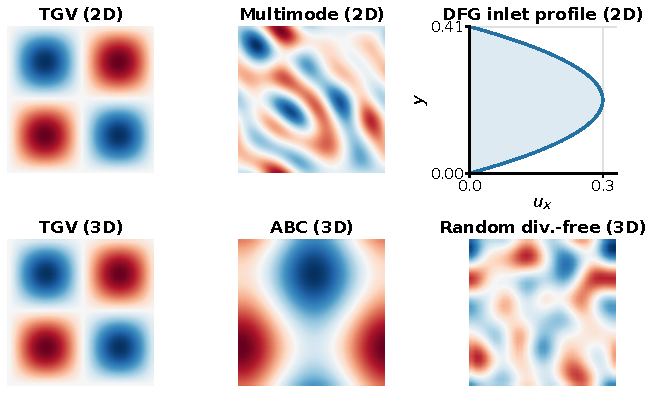
\includegraphics[width=\linewidth]{figures/appendix_ics_ns_combined.pdf}
  \caption{Initial conditions for the F2 and F3 domains (vorticity; 3D shown as $z{=}0$ slice).}
  \label{fig:app:ics_ns}
\end{figure}

\paragraph{Structural mechanics (\cref{fig:app:ics_structural})}
All ICs are material density fields over the beam mesh.
\textbf{Uniform:} $\rho_0 = 0.5$ everywhere.
\textbf{Random:} Gaussian noise centered at $\rho_0=0.5$ ($\sigma=0.3$),
clipped to $[0.05,\,0.95]$.
\textbf{Two density bumps:} two Gaussian pillars ($\rho_\text{peak}=0.95$,
$\sigma=0.12\,L$) at $x=0.35\,L_x$ and $x=0.75\,L_x$, on a soft
background ($\rho_\text{bg}=0.1$).

\begin{figure}
  \centering
  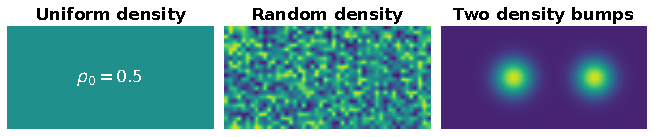
\includegraphics[width=\linewidth]{figures/appendix_ics_structural_mesh.pdf}
  \caption{Initial conditions for the structural mechanics domain.}
  \label{fig:app:ics_structural}
\end{figure}

\paragraph{Heat transfer (\cref{fig:app:ics_thermal})}
All ICs are conductivity or source fields over the thermal mesh.
\textbf{Uniform conductivity:} $k_0 = 0.5$ everywhere.
\textbf{Random conductivity:} Gaussian noise centered at $k_0=0.5$
($\sigma=0.3$), clipped to $[0.05,\,0.95]$.
\textbf{Gaussian source:} single heat source centered at
$(0.5\,L_x,\,0.5\,L_y)$ with width $\sigma=0.2\,\min(L_x,L_y)$.
\textbf{Two-Gaussian conductivity:} ground-truth field for the conductivity
recovery task; two Gaussian peaks at $(0.3\,L_x,\,0.5\,L_y)$ and
$(0.7\,L_x,\,0.5\,L_y)$ with width $\sigma=0.15\,\min(L_x,L_y)$.

\begin{figure}
  \centering
  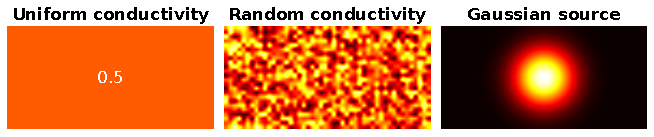
\includegraphics[width=\linewidth]{figures/appendix_ics_thermal_mesh.pdf}
  \caption{Initial conditions for the heat transfer domain.}
  \label{fig:app:ics_thermal}
\end{figure}

\subsection{Cost}
\label{app:cost}

\Cref{fig:app:scaling,fig:app:scaling:fem} show forward time, VJP time, and VJP/forward ratio against element count for all four domains.
A single integer $N$ sets the size:
F2 uses an $N\times N$ grid ($N\in\{64,128,192,256\}$, $4\text{k}$--$66\text{k}$ cells);
F3 an $N\times N\times N$ grid ($N\in\{16,32,48,64,96,128\}$, $4\text{k}$--$2.1\text{M}$ cells);
S an $N\times 2\times\lfloor N/2\rfloor$ hexahedral mesh ($N\in\{4,\ldots,128\}$, $16$--$16\text{k}$ elements);
and H an $N\times\lfloor N/2\rfloor\times 1$ hexahedral mesh ($N\in\{16,\ldots,1024\}$, $128$--$524\text{k}$ elements).
\Cref{tab:merged} reports wall times at $N=64$ (F2), $N=32$ (F3), $N=128$ (S), and $N=256$ (H).
The rollout-length sweeps run F2 at $N=128$ for 10--1000 steps and F3 at $N=48$ for 10--2000 steps.

The fixed RPC overhead (host serialization and HTTP round-trip) adds approximately 2--20\,ms per call and is visible as a floor for the fastest solvers at small problem sizes.
A line that ends before the full size range means that the solver raised an exception (typically an out-of-memory error) or that its first trial exceeded the 1\,000\,s per-trial wall limit; larger sizes are then skipped.
The underlying Tesseract request times out separately after 7\,200\,s.
Forward times span several orders of magnitude across solver families at identical resolution, reflecting differences in algorithmic complexity and hardware target (CPU vs.\ GPU).
Three points need care when reading the curves. Warp-NS's times spike at sizes that are not powers of two ($N=192$ on F2, $N=48$ and 96 on F3).
OpenFOAM's F3 forward times at $N\geq64$ are 1.5--3$\times$ longer than in a rehearsal of the run, and back-to-back measurements attribute the difference to load on the host rather than to the solver image.
PICT's F3 VJP at $N=128$ ended when its container exited after two of three trials.

The VJP request includes a forward pass, so a ratio near~2 means that the gradient costs about one adjoint solve of the forward's cost.
On the NS domains, Exponax, JAX-CFD, and PICT keep a nearly constant ratio across grid sizes, whereas XLB's rises (F2 2.2 to 4.1, F3 1.9 to 4.6) and PhiFlow's falls on F2 (5.3 to 3.1).
Along the rollout sweeps, the ratio grows with the number of steps for most NS solvers, most strongly for INS.jl (to 7.1) and XLB (to 7.0) on F3.
On the mesh domains, TopOpt.jl's VJP costs about one forward solve and torch-fem's 1.3--1.6.
Firedrake stays near~2, while FEniCS falls from 4.3 (S) and 3.2 (H) at the smallest sizes to 2.1--2.3, and JAX-FEM from about 2.5 to 1.5--1.8.
Ratios thus move in both directions within each differentiation strategy.

\Cref{fig:horizon_sweep} extends the F3 rollout to 81\,920 steps at $N=20$, one VJP per horizon.
Peak GPU memory is device-wide and excludes the 768\,MiB the driver reserves.
Two memory readings need care: INS.jl's peak is dominated by the CUDA.jl memory pool, and Warp-NS's peak cannot be read against $N$ because its memory pools carry over between sizes.

\begin{figure}
  \centering
  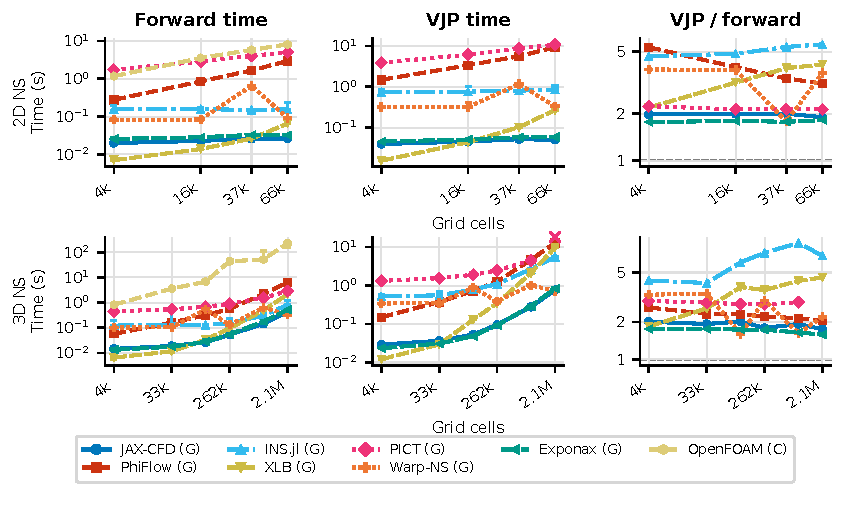
\includegraphics[width=\linewidth]{figures/scaling_ns_combined.pdf}
  \caption{Gradient overhead scaling for the fluid domains (2D NS, top;
    3D NS, bottom). Left: forward time; center: VJP time; right:
    VJP/forward ratio (dashed line marks 1:1). All axes are log-log.
    (G)\,/\,(C) denotes GPU\,/\,CPU execution.}
  \label{fig:app:scaling}
\end{figure}

\begin{figure}
  \centering
  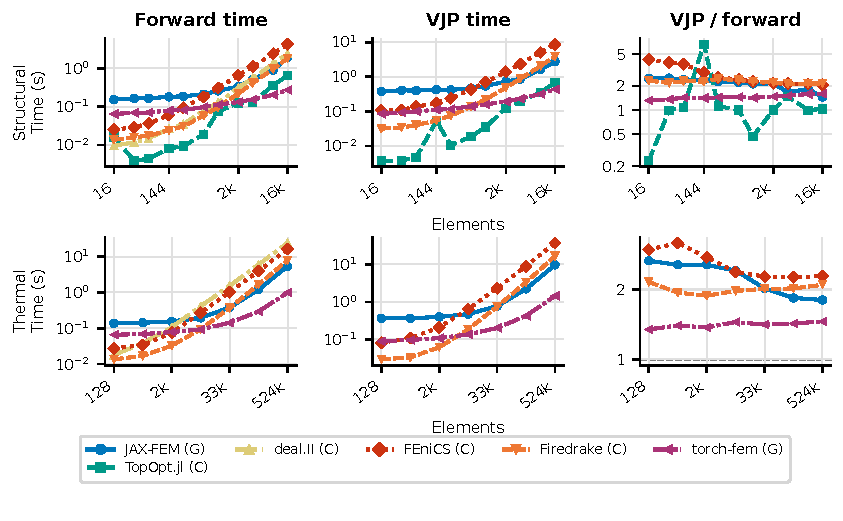
\includegraphics[width=\linewidth]{figures/scaling_fem_combined.pdf}
  \caption{Gradient overhead scaling for the mesh domains (Structural,
    top; Thermal, bottom). Same layout as \cref{fig:app:scaling}.
    deal.II VJP times are omitted (no adjoint).}
  \label{fig:app:scaling:fem}
\end{figure}

\begin{figure}
  \centering
  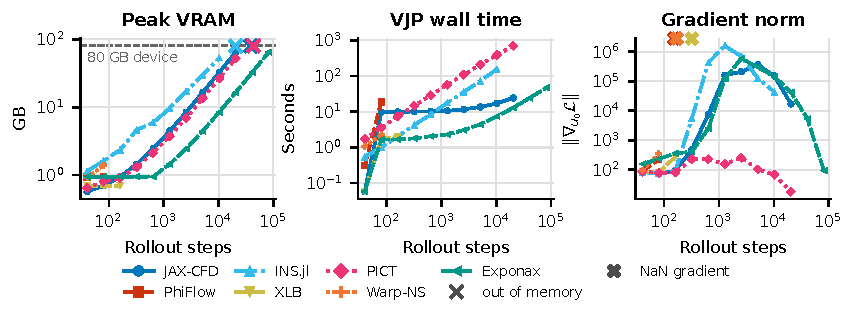
\includegraphics[width=\linewidth]{figures/horizon_sweep_limits.pdf}
  \caption{VJP against rollout length on F3 ($N=20$, $\nu=10^{-3}$, $\Delta t=0.05$): peak GPU memory, wall time, and gradient norm.
    Each line ends at the solver's last successful horizon. Memory failures (out of memory, container exit) are marked at the device limit, and non-finite gradients at the top of the gradient-norm panel.}
  \label{fig:horizon_sweep}
\end{figure}

\subsection{VJP/forward ratios}
\label{app:ratios}

\Cref{tab:app:ratios} lists the ratio of VJP to forward time at the \cref{tab:merged} sizes and its range over each sweep.
Earlier development runs measured far larger ratios, $270\times$ (F2) and $1100\times$ (F3) for XLB and 8--10$\times$ for Exponax and JAX-CFD.
Three causes were found and fixed: the JAX solvers had fallen back to the CPU; the VJP timing counted a second forward solve, because a gradient through tesseract-jax sends a forward request before the VJP request, which recomputes the forward solution; and XLB's checkpointing wrapped single steps rather than blocks of steps, so it stored the full trajectory.
We did not measure how much each fix contributed.
Three cases remain above $5\times$.
INS.jl reaches 5.8--7.8 on F3 at $N\geq48$ and up to 6.2 on F2; we have not established why.
XLB's ratio on F3 rises with the rollout to 7.0 at 2000 steps, plausibly from the recomputation its block checkpointing adds, although we have not verified this.
PhiFlow's 5.3 at F2 $N=64$ falls to 3.1 at $N=256$, consistent with a fixed per-call overhead.
TopOpt.jl's extremes (0.23 and 6.6) come from single slow trials at sub-second times (\cref{app:variance}).

\begin{table}[t]
  \centering\small
  \caption{Ratio of VJP to forward wall time per solver, from median times: at the
    \cref{tab:merged} size, and the range over the grid-size sweep and, for the fluid
    domains, the rollout-length sweep. The VJP request includes a forward pass, so about~2 is
    the typical value for a solver whose gradient costs one adjoint solve.}
  \label{tab:app:ratios}
  \begin{tabular}{@{}l c c c@{}}
    \toprule
    \textbf{Solver} & \textbf{Table size} & \textbf{Grid sweep} & \textbf{Rollout sweep} \\
    \midrule
    \multicolumn{4}{@{}l}{\textit{F2: table size $N=64$; rollout sweep at $N=128$}} \\
      Exponax & 1.8 & 1.8--1.8 & 1.5--1.9 \\
      INS.jl & 4.7 & 4.7--5.6 & 4.1--6.3 \\
      JAX-CFD & 2.0 & 1.9--2.0 & 1.3--2.3 \\
      PhiFlow & 5.3 & 3.1--5.3 & 3.4--5.2 \\
      PICT & 2.2 & 2.1--2.2 & 2.1--2.3 \\
      Warp-NS & 3.8 & 1.8--3.8 & 2.9--4.5 \\
      XLB & 2.2 & 2.2--4.1 & 1.6--4.3 \\
    \midrule
    \multicolumn{4}{@{}l}{\textit{F3: table size $N=32$; rollout sweep at $N=48$}} \\
      Exponax & 1.8 & 1.6--1.8 & 1.5--2.1 \\
      INS.jl & 4.1 & 4.1--8.6 & 3.8--7.1 \\
      JAX-CFD & 1.9 & 1.7--2.0 & 1.6--2.5 \\
      PhiFlow & 2.3 & 2.0--2.6 & 2.1--2.7 \\
      PICT & 2.9 & 2.8--3.0 & 2.6--2.8 \\
      Warp-NS & 3.4 & 1.6--3.4 & 1.5--1.7 \\
      XLB & 2.6 & 1.8--4.6 & 2.3--7.0 \\
    \midrule
    \multicolumn{4}{@{}l}{\textit{S: table size $n_x=128$}} \\
      FEniCS & 2.1 & 2.1--4.0 & $-$ \\
      Firedrake & 2.1 & 2.1--2.5 & $-$ \\
      JAX-FEM & 1.7 & 1.7--2.5 & $-$ \\
      TopOpt.jl & 1.1 & 0.99--1.2 & $-$ \\
      torch-fem & 1.6 & 1.3--1.6 & $-$ \\
    \midrule
    \multicolumn{4}{@{}l}{\textit{H: table size $n_x=256$}} \\
      FEniCS & 2.2 & 2.2--3.2 & $-$ \\
      Firedrake & 2.0 & 1.9--2.1 & $-$ \\
      JAX-FEM & 2.0 & 1.8--2.6 & $-$ \\
      torch-fem & 1.4 & 1.3--1.5 & $-$ \\
    \bottomrule
  \end{tabular}
\end{table}


\subsection{Timing variance}
\label{app:variance}

\Cref{tab:app:variance} lists the coefficient of variation (CV) of the timed trials per configuration, with the sample standard deviation.
The NS suites take 3 trials per configuration and the mesh suites 10.
Across 513 configurations, the median CV is 2.4\% and 40 configurations exceed 15\%.
Of these 40, 26 belong to the two Julia solvers, TopOpt.jl (12) and INS.jl (14), all at sub-second times, and 3 to OpenFOAM on F3 at $N\geq64$, which host load slowed (\cref{app:cost}).
Dropping the single slowest trial brings 36 of the 40 below 15\%.

\begin{table}[t]
  \centering\footnotesize
  \caption{Run-to-run variation of the timed cost measurements: coefficient of variation (CV,
    sample standard deviation with $n-1$ over the mean of the timed trials) per configuration,
    i.e.\ per solver, cost experiment, and sweep value, with the 3 configurations of
    highest CV per problem.}
  \label{tab:app:variance}
  \begin{tabular}{@{}l r r r >{\raggedright\arraybackslash}p{0.48\linewidth}@{}}
    \toprule
    \textbf{Problem} & \textbf{Configs} & \textbf{Median CV} & \textbf{CV\,>\,15\%} & \textbf{Highest CV} \\
    \midrule
      F2 & 135 & 1.6\% & 7 & INS.jl fwd 100 steps (65\%); INS.jl fwd 50 steps (41\%); INS.jl fwd $N=256$ (27\%) \\
      F3 & 174 & 1.5\% & 12 & INS.jl fwd $N=32$ (99\%); INS.jl fwd 50 steps (73\%); INS.jl fwd 10 steps (62\%) \\
      S & 132 & 3.9\% & 20 & TopOpt.jl VJP $n_x=12$ (275\%); TopOpt.jl fwd $n_x=4$ (244\%); TopOpt.jl fwd 1 step (212\%) \\
      H & 72 & 3.4\% & 1 & FEniCS fwd $n_x=16$ (17\%); FEniCS VJP 1 step (11\%); FEniCS VJP $n_x=64$ (10\%) \\
    \midrule
      All & 513 & 2.4\% & 40 & \\
    \bottomrule
  \end{tabular}
\end{table}


\subsection{Outcomes of the \texorpdfstring{16\,GB}{16 GB} failures}
\label{app:outcomes}

\Cref{tab:app:outcomes} lists every configuration that failed on a 16\,GB GPU, in the V100 submission run or the T4 CI run, together with its outcome on the A100.
Every NS configuration that failed on 16\,GB from lack of memory, by losing its container, or without a recorded reason completes on 80\,GB, apart from two solvers no longer in the suite, while the non-finite gradients of the F3 horizon sweep recur.
The longer sweeps then reach new limits, listed in the lower part of the table.
For the mesh domains, the table gives the A100 outcome where the run covers the configuration.

\begin{table}[p]
  \centering\scriptsize
  \setlength{\tabcolsep}{3pt}
  \caption{Configurations that failed on a 16\,GB GPU, in the V100 submission run or the T4
    CI run, and their outcome on the A100 80\,GB. Sizes are $N$ or $n_x$ for the size sweeps and
    rollout steps for the \emph{steps} and \emph{horizon} sweeps. The V100 run stored most
    failures without a reason (\emph{no reason}). \emph{skipped}: not attempted after an
    earlier failure in the same sweep; \emph{died}: the container exited; \emph{not in sweep}:
    outside the sweep range of the A100 run. Memory is the largest peak over the successful
    points, VRAM for GPU solvers and host RAM for CPU solvers, with 1\,GB = $2^{30}$ bytes.
    FEniCS-NS and SU2 are no longer part of the suite. \Cref{tab:app:a100failures} lists
    the failure points of the A100 run.}
  \label{tab:app:outcomes}
  \begin{tabular}{@{}l l l >{\raggedright\arraybackslash}p{0.33\linewidth} >{\raggedright\arraybackslash}p{0.33\linewidth}@{}}
    \toprule
    & \textbf{Sweep} & \textbf{Solver} & \textbf{16\,GB failures} & \textbf{A100 outcome} \\
    \midrule
      F2 & fwd, size & SU2 & V100: 192--256 no reason & solver not in suite \\
      F2 & VJP, size & FEniCS-NS & V100: 128--256 no reason & solver not in suite \\
      F2 & VJP, size & PhiFlow & V100: 192--256 no reason & ok 192--256 (2.6\,GB) \\
      F2 & VJP, size & XLB & V100: 192--256 no reason & ok 192--256 (1.4\,GB) \\
      F2 & VJP, steps & FEniCS-NS & V100: 50--1000 no reason & solver not in suite \\
      F2 & VJP, steps & JAX-CFD & V100: 1000 no reason & ok 1000 (3.7\,GB) \\
      F2 & VJP, steps & PhiFlow & V100: 10--1000 no reason & ok 10--1000 (4.5\,GB) \\
      F2 & VJP, steps & PICT & V100: 1000 no reason & ok 1000 (4.4\,GB) \\
      F2 & VJP, steps & XLB & V100: 10--1000 no reason & ok 10--1000 (0.95\,GB) \\
    \midrule
      F3 & VJP, size & INS.jl & T4: 96 OOM, 128 skipped & ok 96--128 (79\,GB) \\
      F3 & VJP, size & JAX-CFD & T4: 128 OOM & ok 128 (28\,GB) \\
      F3 & VJP, size & PhiFlow & T4: 96 OOM, 128 skipped & ok 96--128 (68\,GB) \\
      F3 & VJP, size & PICT & T4: 96 OOM, 128 skipped & ok 96 (43\,GB); died 128 \\
      F3 & VJP, size & Warp-NS & T4: 96 OOM, 128 skipped & ok 96--128 (58\,GB) \\
      F3 & VJP, size & XLB & V100: 48--64 no reason; T4: 128 OOM & ok 48--128 (44\,GB) \\
      F3 & VJP, steps & Exponax & T4: 2000 OOM & ok 2000 (30\,GB) \\
      F3 & VJP, steps & INS.jl & T4: 500 OOM, 1000--2000 skipped & ok 500--1000 (79\,GB); OOM 2000 \\
      F3 & VJP, steps & JAX-CFD & T4: 1000 OOM, 2000 skipped & ok 1000 (52\,GB); OOM 2000 \\
      F3 & VJP, steps & PhiFlow & V100: 10--100 no reason; T4: 500 OOM, 1000--2000 skipped & ok 10--1000 (65\,GB); OOM 2000 \\
      F3 & VJP, steps & PICT & T4: 500--2000 died & ok 500--2000 (74\,GB) \\
      F3 & VJP, steps & Warp-NS & T4: 500 OOM, 1000--2000 skipped & ok 500 (72\,GB); OOM 1000; skipped 2000 \\
      F3 & VJP, steps & XLB & V100: 10--100 no reason & ok 10--100 (2.2\,GB) \\
      F3 & horizon & Exponax & V100: 10240 OOM; T4: 20480 OOM, 40960--81920 skipped & ok 10240--81920 (64\,GB) \\
      F3 & horizon & INS.jl & T4: 5120 OOM, 10240--81920 skipped & ok 5120--10240 (53\,GB); OOM 20480; skipped 40960--81920 \\
      F3 & horizon & JAX-CFD & T4: 10240 OOM, 20480--81920 skipped & ok 10240--20480 (64\,GB); OOM 40960; skipped 81920 \\
      F3 & horizon & PhiFlow & V100: 160 NaN, 320--10240 skipped; T4: 160 NaN, 320--81920 skipped & NaN 160; skipped 320--81920 \\
      F3 & horizon & PICT & V100: 5120 OOM, 10240 skipped; T4: 10240 died, 20480--81920 skipped & ok 5120--20480 (52\,GB); died 40960; skipped 81920 \\
      F3 & horizon & Warp-NS & V100: 160 NaN, 320--10240 skipped; T4: 160 NaN, 320--81920 skipped & NaN 160; skipped 320--81920 \\
      F3 & horizon & XLB & V100: 160 OOM, 320--10240 skipped; T4: 320 NaN, 640--81920 skipped & ok 160 (0.7\,GB); NaN 320; skipped 640--81920 \\
    \midrule
      S & fwd, size & deal.II & V100: 256--3200 no reason & not in sweep 256--3200 \\
      S & fwd, size & FEniCS & V100: 256--3200 no reason & not in sweep 256--3200 \\
      S & fwd, size & Firedrake & V100: 256 error, 512--3200 no reason & not in sweep 256--3200 \\
      S & fwd, size & JAX-FEM & V100: 512--3200 no reason & not in sweep 512--3200 \\
      S & fwd, size & TopOpt.jl & V100: 1024--3200 no reason & not in sweep 1024--3200 \\
      S & VJP, size & deal.II & V100: 2048 timeout, 3200 no reason & excluded \\
      S & VJP, size & FEniCS & V100: 512 error, 1024--3200 no reason & not in sweep 512--3200 \\
      S & VJP, size & Firedrake & V100: 256 error, 512--3200 no reason & not in sweep 256--3200 \\
      S & VJP, size & JAX-FEM & V100: 512 error, 1024--3200 no reason & not in sweep 512--3200 \\
      S & VJP, size & TopOpt.jl & V100: 2048 timeout, 3200 no reason & not in sweep 2048--3200 \\
    \midrule
      H & fwd, size & deal.II & V100: 2048--4500 no reason & not in sweep 2048--4500 \\
      H & fwd, size & FEniCS & V100: 1024--4500 no reason & ok 1024 (4.6\,GB); not in sweep 2048--4500 \\
      H & fwd, size & Firedrake & V100: 512 error, 1024--4500 no reason & ok 512--1024 (5.6\,GB); not in sweep 2048--4500 \\
      H & fwd, size & JAX-FEM & V100: 2048--4500 no reason & not in sweep 2048--4500 \\
      H & fwd, size & torch-fem & V100: 2048 OOM, 4500 no reason & not in sweep 2048--4500 \\
      H & VJP, size & deal.II & V100: 2048 timeout, 4500 no reason & excluded \\
      H & VJP, size & FEniCS & V100: 1024 error, 2048--4500 no reason & ok 1024 (4.8\,GB); not in sweep 2048--4500 \\
      H & VJP, size & Firedrake & V100: 512 error, 1024--4500 no reason & ok 512--1024 (7.7\,GB); not in sweep 2048--4500 \\
      H & VJP, size & JAX-FEM & V100: 2048 error, 4500 no reason & not in sweep 2048--4500 \\
      H & VJP, size & torch-fem & V100: 2048 OOM, 4500 no reason & not in sweep 2048--4500 \\
    \bottomrule
  \end{tabular}
\end{table}

\begin{table}[t]
  \centering\small
  \caption{Failure points of the A100 run in the fluid cost and horizon sweeps, with the
    peak VRAM recorded before the failure (an allocation that does not fit is not counted;
    1\,GB = $2^{30}$ bytes). Larger points of the same sweep were not attempted.}
  \label{tab:app:a100failures}
  \begin{tabular}{@{}l l l l l r@{}}
    \toprule
    & \textbf{Sweep} & \textbf{Solver} & \textbf{First failure} & \textbf{Outcome} & \textbf{VRAM (GB)} \\
    \midrule
      F3 & VJP, size & PICT & $N=128$ & died & 79 \\
      F3 & VJP, steps & INS.jl & 2000 steps & OOM & 79 \\
      F3 & VJP, steps & JAX-CFD & 2000 steps & OOM & 52 \\
      F3 & VJP, steps & PhiFlow & 2000 steps & OOM & 65 \\
      F3 & VJP, steps & Warp-NS & 1000 steps & OOM & 79 \\
      F3 & horizon & INS.jl & 20480 steps & OOM & 79 \\
      F3 & horizon & JAX-CFD & 40960 steps & OOM & 64 \\
      F3 & horizon & PhiFlow & 160 steps & NaN & 1.5 \\
      F3 & horizon & PICT & 40960 steps & died & 79 \\
      F3 & horizon & Warp-NS & 160 steps & NaN & 2.3 \\
      F3 & horizon & XLB & 320 steps & NaN & 0.7 \\
    \bottomrule
  \end{tabular}
\end{table}


\subsection{Physical accuracy}
\label{app:physical_accuracy}

As a basic sanity check, we run agreement and baseline experiments on each NS domain: agreement measures relative $\ell_2$ error vs.\ the analytic TGV solution across a $\nu$ sweep at fixed resolution, and baseline measures convergence with resolution at one timestep.
All solvers that support the periodic TGV domain pass both checks with errors below $10^{-2}$.

\paragraph{F2 cylinder-flow forward accuracy}
The F2 domain uses a cylinder obstacle in a channel.
Unlike the periodic TGV, no analytic solution exists, so solvers are compared against the cross-solver consensus (mean over valid solvers).
This experiment uses a unit-square domain $[0,1]^2$ with a cylinder at $(0.5, 0.5)$, radius $0.1$, $N=64$, 500 steps at $\Delta t=0.01$; the physical accuracy sweeps below use the full channel domain $[0,8]\times[0,2]$. The F2 drag-optimization convergence experiment (\cref{app:effort}) uses the same unit-square domain but a smaller cylinder (radius $0.05$, $D=0.1$), which sets $\text{Re}=U D/\nu=20$ at the fixed $U=0.5$, $\nu=0.0025$ used there; both setups are F2 cylinder-channel flows but exercise different aspects of the benchmark.
Three solvers (JAX-CFD, INS.jl, Warp-NS) produce invalid results on this geometry due to boundary condition incompatibilities.
\Cref{fig:app:cylinder} shows consensus error vs.\ $\nu$ and final vorticity fields for the four solvers that run successfully.

\begin{figure}
  \centering
  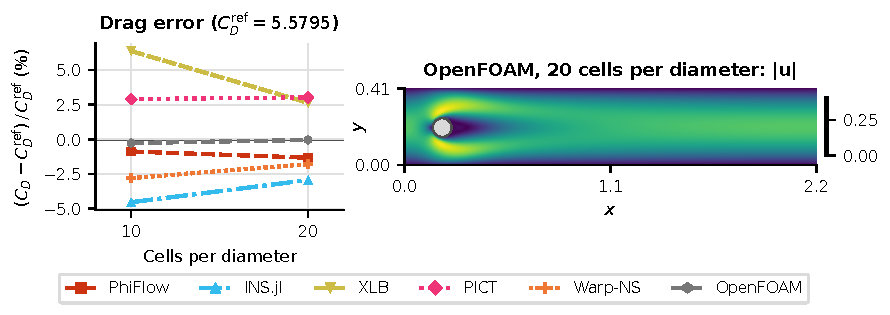
\includegraphics[width=\linewidth]{figures/appendix_cylinder.pdf}
  \caption{F2 cylinder-flow forward accuracy: relative $\ell_2$ error vs.\ the cross-solver consensus as a function of $\nu$ at $N=64$, 500 steps (left), and final vorticity fields at $\nu=0.01$ (right). Solvers that fail on this geometry are omitted.}
  \label{fig:app:cylinder}
\end{figure}

\paragraph{Physical accuracy sweeps}
For the two fluid domains, \cref{fig:app:pa_ns2d,fig:app:pa_ns3d} show resolution~$N$, viscosity~$\nu$, and rollout length against three physical metrics.
F2 uses the $[0,8]\times[0,2]$ cylinder-channel at Re\,=\,20, sweeping $N\in\{16,32,64,128\}$, $\nu\in\{0.001,0.005,0.01,0.05,0.1\}$, and up to 100 steps.
F3 uses the $[0,2\pi]^3$ TGV box at $N=16$, sweeping $\nu\in\{0.001,0.01,0.05,0.1\}$ and up to 50 steps.
\textbf{Analytic TGV error} is the relative $\ell_2$ error against the Taylor--Green vortex closed-form solution. Lower is better, with values below $10^{-2}$ indicating good accuracy.
\textbf{Divergence RMS} measures how strongly the solver violates the incompressibility constraint $\nabla \cdot \mathbf{u} = 0$. For a well-posed incompressible solver this should be near machine precision ($\lesssim 10^{-6}$), while values above $10^{-2}$ indicate a solver that does not enforce incompressibility exactly (e.g.\ LBM methods).
\textbf{Kinetic energy} is the domain-averaged $\frac{1}{2}\|\mathbf{u}\|^2$.
For 2D NS the analytical ground truth is $\mathrm{KE}(t) = \tfrac{1}{4}e^{-4\nu t}$, shown as a dashed reference line, and solvers should track it closely.
For 3D NS no closed-form solution exists, so all solvers should at least agree with each other; spread at a given parameter value indicates a physical accuracy problem.
Solvers that enforce the divergence-free constraint exactly at each step by construction (PhiFlow, Warp-NS, PICT, JAX-CFD, INS.jl, Exponax) sit at or near machine precision regardless of resolution or viscosity.
XLB exhibits a compressibility floor in divergence RMS and analytic error that is largely independent of $\nu$ or resolution, consistent with the $O(\mathrm{Ma}^2)$ compressibility error inherent to the LBM formulation.

For the mesh domains, all structural and thermal solvers agree to machine precision across the full load range, consistent with the expected $C \propto F^2$ scaling of linear compliance.

\begin{figure}
  \centering
  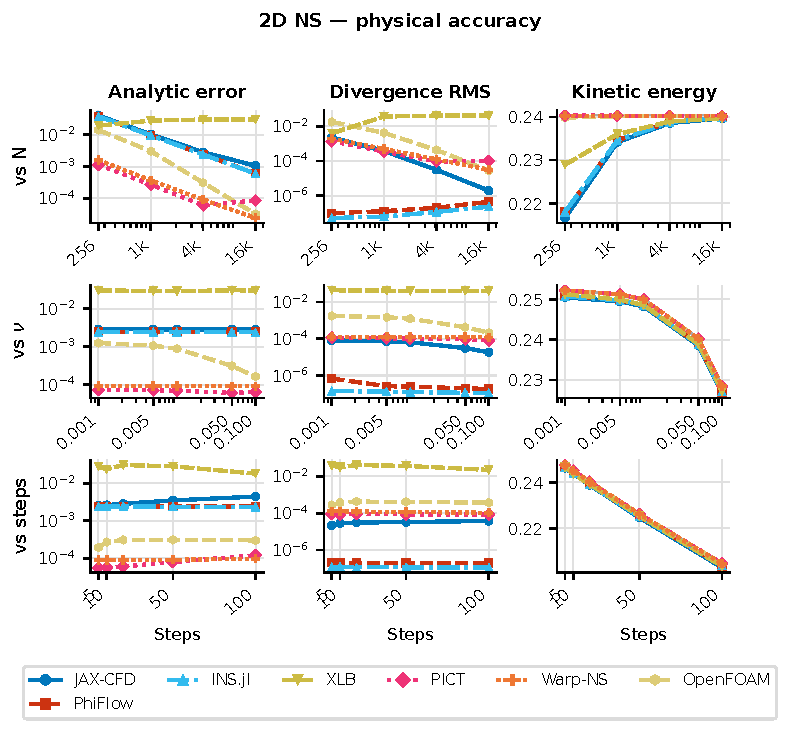
\includegraphics[width=\linewidth]{figures/appendix_pa_ns2d.pdf}
  \caption{2D NS physical accuracy. Each panel sweeps one parameter (resolution, $\nu$, or steps) on the x-axis against one physical metric on the y-axis.}
  \label{fig:app:pa_ns2d}
\end{figure}

\begin{figure}
  \centering
  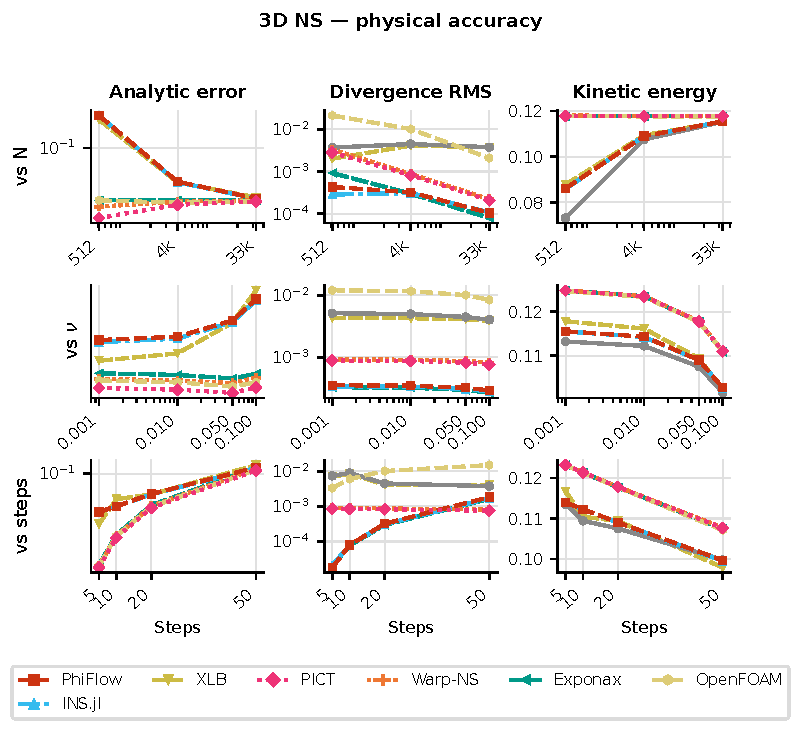
\includegraphics[width=\linewidth]{figures/appendix_pa_ns3d.pdf}
  \caption{3D NS physical accuracy on the triply-periodic TGV domain $[0,2\pi)^3$.
    Rows sweep resolution $N$ (top), viscosity $\nu$ (middle), and rollout length (bottom).
    Columns report analytic TGV error, divergence RMS, and kinetic energy.
    No closed-form kinetic-energy reference exists for 3D NS, so solvers are compared
    against each other; spread at a given parameter value indicates a physical accuracy
    discrepancy.}
  \label{fig:app:pa_ns3d}
\end{figure}

\subsection{Gradient quality}
\label{app:gradient}

\paragraph{Finite-difference verification}
\Cref{fig:app:fdcheck} extends the FD verification from \cref{sec:quality} to all four domains.
The U-shaped error curve (truncation error at large~$\varepsilon$, floating-point roundoff at small~$\varepsilon$) is visible in every domain and for every solver that provides gradients.
The best~$\varepsilon$ lies between 0.1 and 5 for the NS solvers and between 0.003 and 0.03 for the mesh solvers' density gradients, and every differentiable solver reaches a cosine similarity above $0.999\,999\,9$ at its best~$\varepsilon$.

\begin{figure}
  \centering
  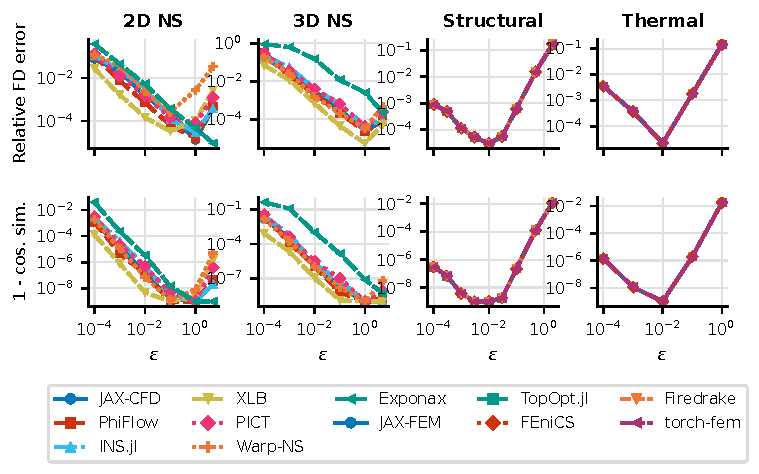
\includegraphics[width=\linewidth]{figures/appendix_fd_check.pdf}
  \caption{FD gradient verification across all four domains.
    Top row: relative $\ell_2$ error vs.\ perturbation size~$\varepsilon$.
    Bottom row: subspace cosine similarity vs.~$\varepsilon$.}
  \label{fig:app:fdcheck}
\end{figure}

\begin{figure}
  \centering
  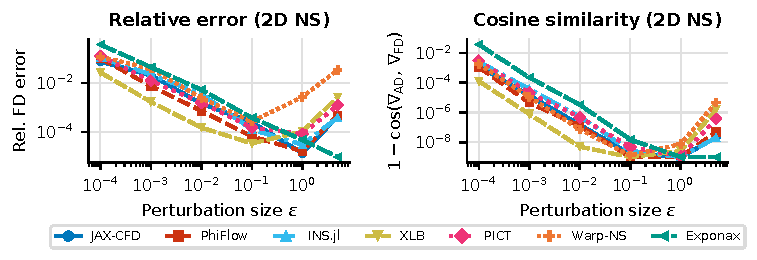
\includegraphics[width=0.85\linewidth]{figures/fd_check.pdf}
  \caption{FD gradient verification on the 2D NS domain (focused view of the leftmost column of \cref{fig:app:fdcheck}).
    Relative $\ell_2$ error (left) and cosine similarity (right) vs.\ perturbation size~$\varepsilon$, normalized by the RMS magnitude of the initial condition.
    The best~$\varepsilon$ lies between 0.1 and 5.}
  \label{fig:app:fdcheck:ns2d}
\end{figure}

\paragraph{Exact-gradient checks}
On F2, two checks compare against the exact Taylor--Green solution at $N=32$ after 20 steps of $\Delta t=0.05$, for $\nu\in\{0.001,0.005,0.01,0.02,0.05\}$.
The first compares the gradient of $J=\sum|\mathbf{u}(T)|^2$ with respect to the initial field against $\nabla J = 2e^{-4\nu T}\mathbf{u}_0$, after projecting out the gradient's curl-free part, since the closed form holds for divergence-free perturbations.
The second compares $\mathrm{d}J/\mathrm{d}\nu$ against $-4TJ$.
Neither needs a step size, but both include the forward discretization error.
Exponax represents the Taylor--Green mode exactly, and its errors of about $10^{-5}$ are consistent with float32 roundoff.
JAX-CFD, PhiFlow, and INS.jl average the collocated input onto their staggered grids and back, which scales the mode by $\cos^2(\Delta x/2)$, a factor the gradient picks up twice. At $N=32$ this accounts for their shared initial-state error of $1.9\times10^{-2}$; their viscosity errors also coincide, at $2.2\times10^{-2}$.
XLB's initial-state error grows with~$\nu$ from $7\times10^{-5}$ to $8\times10^{-4}$, Warp-NS's stays near $5\times10^{-3}$, and PICT's grows from $4\times10^{-3}$ to $2\times10^{-2}$; PICT's viscosity error reaches $5.4\times10^{-2}$ at $\nu=0.001$.
All solvers pass the checks' thresholds (error at most 0.1 and within $3\times$ the peer median), which are provisional.
\Cref{tab:gradchecks} reports the errors at $\nu=0.01$.

\paragraph{Jacobian singular value spectra}
\Cref{fig:app:svd2d} shows normalized singular value spectra $\sigma_i/\sigma_0$ of the solver Jacobian for 2D NS across rollout length and viscosity; the 3D NS spectra appear in \cref{fig:conditioning}.
Faster spectral decay indicates a more ill-conditioned Jacobian.
Rollout length and viscosity change individual condition numbers by up to two orders of magnitude without a consistent direction, while the ordering of the solvers stays the same in every configuration: in 2D, XLB has the smallest condition number (20--48), followed by PICT ($2\times10^5$--$2\times10^6$), with the other solvers between $2\times10^7$ and $10^{11}$.
Exponax, which solves the 2D problem in vorticity form, joins the projection solvers at about $10^{10}$ there, unlike in 3D. This is consistent with attributing the drop-off to non-solenoidal velocity modes~\citep{guermond2006overview,bhatia2013helmholtz}, since the vorticity form discards the curl-free part of its input.

\begin{figure}
  \centering
  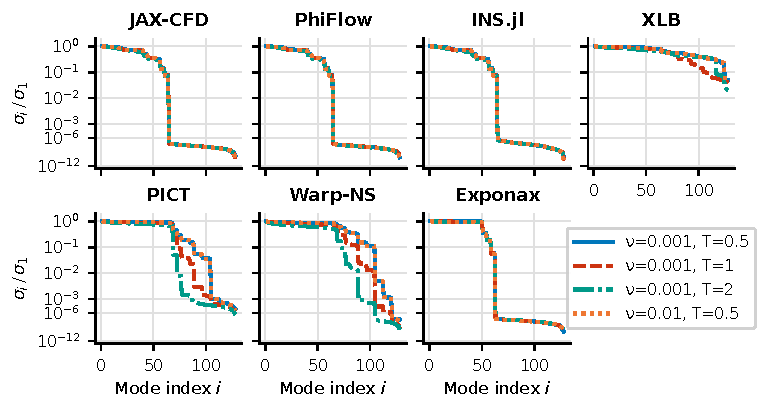
\includegraphics[width=\linewidth]{figures/appendix_jacobian_svd_2d.pdf}
  \caption{Normalized Jacobian singular value spectra for 2D NS.
    Each panel shows a different $(\nu, T)$ configuration.
    Faster decay corresponds to a more ill-conditioned Jacobian.}
  \label{fig:app:svd2d}
\end{figure}

\paragraph{Gradient quality over rollout length}
\Cref{fig:app:horizon} shows how FD agreement evolves with rollout length on F2 ($N=16$, 5 to 320 steps).
The best relative FD error grows from $3\times10^{-6}$--$4\times10^{-5}$ at 5 steps to $2\times10^{-4}$--$6\times10^{-4}$ at 320 steps, and $1-{}$cosine stays below $10^{-7}$ throughout, so no solver loses gradient accuracy within this range.
The growth does not follow the conditioning: XLB, the best-conditioned solver, ends within the range of the others.
For several solvers, the best~$\varepsilon$ moves from 1 to 0.1 at the longest rollouts.

\begin{figure}
  \centering
  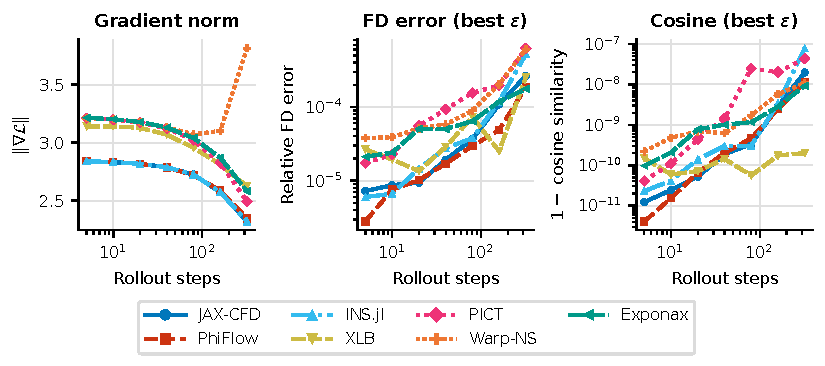
\includegraphics[width=\linewidth]{figures/horizon_sweep.pdf}
  \caption{Gradient quality vs.\ rollout length (2D NS).
    Left: gradient norm.
    Middle: best FD relative error over~$\varepsilon$.
    Right: $1-{}$cosine similarity at the best~$\varepsilon$.}
  \label{fig:app:horizon}
\end{figure}

\paragraph{FD U-curves}
\Cref{fig:app:ucurves_f2} shows the full FD U-curves (relative error vs.\ perturbation size~$\varepsilon$) at each rollout length on F2.
Each U-curve has a characteristic minimum: too-small $\varepsilon$ is dominated by floating-point cancellation, and too-large $\varepsilon$ by nonlinear truncation error.
The minimum generally rises as the rollout grows.

\begin{figure}
  \centering
  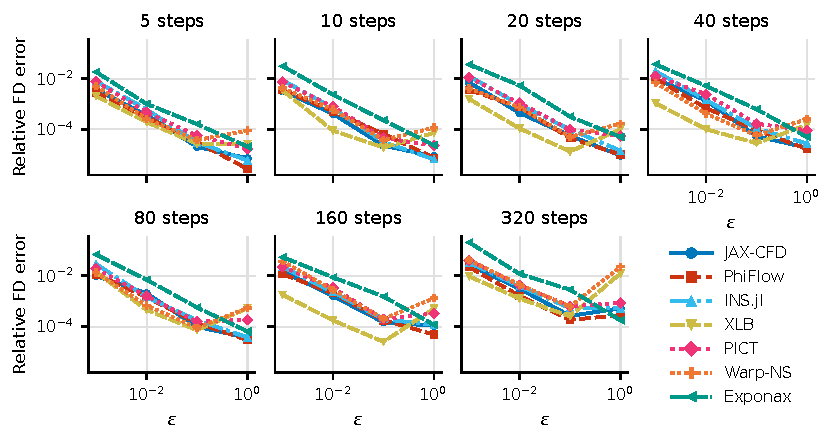
\includegraphics[width=\linewidth]{figures/appendix_ucurves_f2.pdf}
  \caption{FD U-curves for F2 (2D NS): relative FD error vs.\ perturbation size~$\varepsilon$ at each rollout length~$T$.}
  \label{fig:app:ucurves_f2}
\end{figure}

\subsection{Forced Kolmogorov flow}
\label{app:kolmogorov}

\paragraph{Setup}
F2's second setup is forced turbulence on the periodic box $[0,2\pi)^2$,
$\partial_t\mathbf{u} + (\mathbf{u}\cdot\nabla)\mathbf{u} = -\nabla p
+ \nu\nabla^2\mathbf{u} + \mathbf{f} - \alpha\mathbf{u}$,
$\nabla\cdot\mathbf{u} = 0$, with the body force $\mathbf{f} = (A\sin\kappa y, 0)$, $A = 1$, $\kappa = 4$,
linear drag $\alpha = 0.1$ and $\nu = 2\times10^{-3}$.
The drag removes the energy that the 2D inverse cascade accumulates at the
largest scales, so the flow settles into a chaotic, statistically steady state.
A $64^2$ grid resolves it only roughly: it departs from a $4\times$ finer run by
about 2\% every 0.1 time units.

\paragraph{Forcing inputs}
The F2 interface gains two optional inputs, a cell-centered force field and a
drag coefficient. They are accepted only on periodic 2D boxes and are not
differentiated. Each solver applies them inside its own time step, in both the
forward pass and the VJP, and maps the force to its native grid locations the
same way it maps the initial condition (\cref{tab:app:forcing}).
With a force, XLB sizes its lattice Mach number from a bound that does not
depend on the solution, so a flow spun up from rest stays at the target Mach
number. Without the new inputs, every solver runs its previous code: on
unforced Taylor--Green and multimode flows, JAX-CFD, XLB and INS.jl reproduce
their previous outputs bit for bit, and the other solvers agree to within the
run-to-run variation of the unchanged code.

\begin{table}[h]
  \centering\small
  \caption{How each solver applies the Kolmogorov force and the linear drag.}
  \label{tab:app:forcing}
  \begin{tabular}{@{}lll@{}}
    \toprule
    \textbf{Solver} & \textbf{Force} & \textbf{Drag} \\
    \midrule
    JAX-CFD & forcing callable, averaged onto the faces & explicit, every RK4 stage \\
    PhiFlow & resampled to the faces, every RK4 stage & every RK4 stage \\
    INS.jl & projected staggered force in the right-hand side & every RK4 stage \\
    XLB & exact-difference method after collision & semi-implicit, half-force velocity \\
    PICT & velocity source, set every step & explicit, start of step \\
    Warp-NS & tentative-velocity kernel & explicit \\
    Exponax & spectral curl of the force, as its injection term & its native drag term \\
    OpenFOAM & \multicolumn{2}{l}{not supported: icoFoam has no momentum source term} \\
    \bottomrule
  \end{tabular}
\end{table}

\paragraph{Ground truth}
The ground truth is an Exponax run at $1024^2$ (ETDRK2 with 2/3-rule dealiasing,
CFL number about 0.1) from eight states, each spun up from a random field for
100 time units at $512^2$. A $512^2$ run from the same state differs from it by
0.3\% after one time unit and by 2.3--3.2\% after four, at a vorticity
correlation of at least 0.997. It stays above 0.95 correlation for 6.5 to 7.5
time units, beyond the scored horizon of four. As an independent check, JAX-CFD
converges to the truth at observed orders 1.6 and 1.9 between $64^2$ and
$256^2$, down to the 0.3\% floor at $512^2$. Three of the eight states are the
test states of the checks below.

\paragraph{Checks}
\textit{Laminar forcing} (\texttt{forward/kolmogorov\_laminar}). From rest at
$\nu = 0.05$, the flow stays a shear flow whose advection term vanishes, so
$u = (A/\lambda)(1 - e^{-\lambda t})\sin(\kappa y)$, $v = 0$ with
$\lambda = \nu\kappa^2 + \alpha$ is exact. Solvers run $N \in \{32, 64, 128\}$
to $t = 2$ with a time step small enough that the error is spatial. A solver
passes with at most 5\% error at $N = 64$ and an observed order of at least
0.8. A correct second-order scheme misses by about 1\% at $N = 64$, while a
convention error (a missing $2\pi/L$, a flipped sign, a force half a cell off)
misses by 20\% or more.

\textit{Turbulent forward accuracy} (\texttt{forward/kolmogorov}). Each solver
runs grids from $32^2$ to $256^2$ at the CFL number of $64^2$ with
$\Delta t = 0.01$, from the three test states to $t = 1, 2, 3, 4$, and is scored
on $64^2$ against the truth. It passes if its observed order from $64^2$ to
$256^2$ at $t = 1$ is at least 0.8 and no grid from $64^2$ up diverges. The bound
follows from the scheme's consistency, not from the other solvers.

\textit{Chained gradients} (\texttt{gradient/chain\_fd\_check}). A training
loss compares every interval with a target and normalizes by the target's norm,
so each call in a chain receives a far smaller cotangent than in the single-call
checks. The check chains 16 calls of 0.1 time units at $64^2$, starting from a
test state plus a 1\% divergence-free offset. Its loss is the mean relative
squared distance to the solver's own unperturbed chain. The VJP is compared with
central differences along 8 divergence-free directions at
$\varepsilon \in \{1, 0.1, 0.01\}$. A solver passes with a cosine of at least
0.99, a relative error of at most $10^{-2}$, and an error no more than 50 times
the peer median.

\begin{table}[h]
  \centering\small
  \caption{Kolmogorov-flow checks. \emph{Laminar}: relative error against the
    exact solution at $t = 2$. \emph{Turbulent}: median relative error against
    the ground truth at $t = 1$ on each grid, and the observed order from $64^2$
    to $256^2$. \emph{Chained}: median relative error and cosine of the VJP at
    the best $\varepsilon$. A100, PICT with the fix described below.}
  \label{tab:app:kolmogorov}
  \begin{tabular}{@{}lccc@{}}
    \toprule
    & \multicolumn{3}{c}{\textbf{Laminar error}} \\
    \cmidrule(l){2-4}
    \textbf{Solver} & $N=32$ & $64$ & $128$ \\
    \midrule
    Exponax & 3.0e-6 & 3.5e-5 & 1.3e-5 \\
    JAX-CFD, INS.jl, PhiFlow & 2.9e-2 & 7.4e-3 & 1.8e-3 \\
    PICT & 2.9e-2 & 7.1e-3 & 1.7e-3 \\
    Warp-NS & 3.0e-2 & 7.7e-3 & 2.2e-3 \\
    XLB & 7.8e-2 & 1.9e-2 & 4.8e-3 \\
    \bottomrule
  \end{tabular}

  \vspace{6pt}
  \begin{tabular}{@{}lcccccc@{}}
    \toprule
    & \multicolumn{5}{c}{\textbf{Turbulent error}} & \multicolumn{1}{c}{\textbf{Chained}} \\
    \cmidrule(lr){2-6}\cmidrule(l){7-7}
    \textbf{Solver} & $32^2$ & $64^2$ & $128^2$ & $256^2$ & order & error / cosine \\
    \midrule
    Exponax & 0.168 & 0.039 & 0.0046 & 0.0028 & 1.89 & 1.8e-3 / 1.000 \\
    JAX-CFD & 0.226 & 0.086 & 0.029 & 0.0077 & 1.73 & 2.4e-4 / 1.000 \\
    INS.jl & 0.226 & 0.086 & 0.029 & 0.0077 & 1.73 & 2.0e-4 / 1.000 \\
    XLB & 0.135 & 0.032 & 0.0063 & 0.0032 & 1.66 & 9.8e-5 / 1.000 \\
    PICT & 0.258 & 0.092 & 0.034 & 0.012 & 1.46 & 1.4e-3 / 1.000 \\
    PhiFlow & 0.206 & 0.082 & 0.028 & diverged & $-$ & 5.0e-2 / 0.997 \\
    \bottomrule
  \end{tabular}
\end{table}

\paragraph{Results}
\Cref{tab:app:kolmogorov} lists the results. Every solver passes the laminar
check. Exponax represents the single forced mode exactly, so its laminar error
is float32 round-off. On the turbulent flow, every solver passes both remaining
checks except PhiFlow, which fails both: its $256^2$ run turns non-finite
between $t = 3$ and $t = 4$ from two of the three states, and its finite
differences on the chain change erratically with $\varepsilon$, while every
other solver's agree with its VJP to within 3\% at every $\varepsilon$. We have
not established the cause of either failure. JAX-CFD and INS.jl, which share a
discretization (\cref{tab:solvers}), agree to every printed digit on both
forward checks.

Two solvers are excluded from the turbulent checks. Warp-NS integrates with
explicit Euler and central differences, which is linearly unstable on this flow
unless $\Delta t \lesssim 4\nu/u^2$, a bound that does not shrink with the grid.
OpenFOAM's icoFoam has no momentum source term, and OpenFOAM has no VJP.

\paragraph{PICT's adjoint tolerance}
PICT's linear solves stop once the RMS of their residual falls below an absolute
tolerance, $10^{-5}$ in float32 by default, and its adjoint solves use the same
tolerance. When the cotangent is small, the adjoint residual starts near that
tolerance and the solves stop early, so the VJP is no longer linear in the
cotangent. Single calls with $O(1)$ cotangents are unaffected. On a 16-call
chain with cotangents of about $10^{-4}$ per entry, the gradient with respect to
a state 1, 3, 8 and 16 calls before the loss disagreed with finite differences by
0.04\%, 3.7\%, 10\% and 73\%, and the chained check reported a median error of
0.89 at a cosine of 0.51. The wrapper now scales each cotangent to a largest
entry of one before PICT's backward pass and scales the gradient back, which is
exact for a linear VJP and makes the tolerance relative to the cotangent. This
deviates from PICT's defaults and is documented with the solver.

\subsection{Optimization}
\label{app:recovery}

\paragraph{Optimizer configurations}
The optimization tasks use Adam (\texttt{optax.adam} with the defaults
$\beta_1{=}0.9$, $\beta_2{=}0.999$, $\epsilon{=}10^{-8}$) or SciPy's
L-BFGS-B with its default memory of 10 correction pairs. L-BFGS-B iterates in
float64 and passes each iterate to the solver in the solver's input precision.
Adam stops at the iteration budget or after \emph{patience} iterations without
improving the best loss by more than a relative threshold. L-BFGS-B stops at
the iteration budget, when the gradient's 2-norm falls below $10^{-7}$, or when
its line search fails; SciPy's own convergence tests are disabled. A trial point
with a non-finite loss or gradient is reported to the line search as a worse
loss, so that the line search rejects it. Per-task settings:
\begin{itemize}\itemsep0pt
  \item \textbf{F2 (drag minimization)}: Adam, $\eta{=}10^{-2}$, at most 100
        iterations, stopping once the loss has not dropped by 0.1\% in 10
        iterations. Each iterate is projected onto non-negative inlet profiles
        with the benchmark's flow rate and a peak of at most the benchmark's
        $U_m$.
  \item \textbf{F3 (IC recovery)}: L-BFGS-B with solenoidal gradient
        projection (L-BFGS+proj, next paragraph), 100 iterations, starting from
        $u\equiv 0$, for three targets.
  \item \textbf{S (topology optimization)}: Adam, $\eta{=}5{\times}10^{-2}$,
        2\,500 iterations, patience 100, with a soft volume-fraction penalty
        of weight 50 and densities clipped to $[10^{-3},1]$.
  \item \textbf{H (conductivity recovery)}: L-BFGS-B, 1\,000 iterations, on a
        sigmoid reparametrization that keeps the density in $[10^{-3},1]$ and
        makes the SIMP conductivity affine in the latent variable.
\end{itemize}

\paragraph{Solenoidal gradient projection (F3)}
L-BFGS+proj applies a spectral Helmholtz projection to every gradient the
optimizer sees,
$\hat g^{\mathrm{df}}_i = \hat g_i - k_i (k\!\cdot\!\hat g) / |k|^2$,
where $\hat g$ is the FFT of the gradient on the periodic box. This restricts
the search direction to divergence-free fields. The projection is implemented
once in the harness and applied uniformly to all seven fluid solvers; we do not
project elsewhere because the divergence-free constraint is specific to the
incompressible NS state.

\paragraph{2D drag minimization}
\Cref{fig:app:dragopt} shows the drag minimization on the DFG 2D-1 channel at
Re\,=\,20 with 10 cells per cylinder diameter, run to $t=4$, by which time the
drag coefficient $C_d$ is within 0.1\% of its steady value at this resolution.
The loss is $C_d/C_{d,0}$, where $C_{d,0}$ is the drag of the benchmark's
parabolic inlet profile. From initial drag coefficients of 5.3--5.9, all five
solvers that run the channel reduce drag by 46--48\% in 44--69 iterations:
INS.jl by 48.0\%, PhiFlow by 47.7\%, XLB by 47.1\%, PICT by 46.8\%, and
Warp-NS by 46.3\%. Their loss levels off after 27--34 iterations.
Exponax represents only periodic fields, and JAX-CFD~0.2.1 cannot express the
channel's inflow, outflow, and obstacle through its API
(\cref{app:solver-issues}).

\begin{figure}
  \centering
  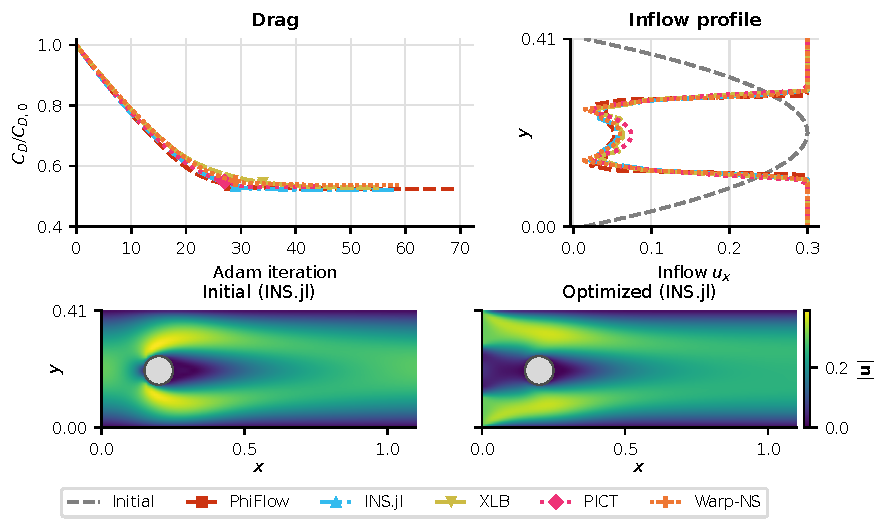
\includegraphics[width=\linewidth]{figures/drag_opt_re20.pdf}
  \caption{2D drag minimization on the DFG 2D-1 channel at Re\,=\,20.
    Top left: $C_d/C_{d,0}$ per Adam iteration, with a dot where the loss
    levels off. Top right: initial and optimized inlet profiles. Bottom:
    velocity magnitude near the cylinder before and after optimization for
    the solver with the largest drag reduction.}
  \label{fig:app:dragopt}
\end{figure}

\paragraph{3D NS IC recovery}
The task starts from a zero velocity field on a $16^3$ grid of the
$[0,2\pi)^3$ periodic box and recovers the initial state of a 100-step rollout
($\nu=0.01$, $\Delta t=0.02$) by minimizing the $\ell_2$ distance to the target
final state. We report the \emph{IC error}
$\|\mathbf{u}^{*}_0 - \mathbf{u}_0\|_2 / \|\mathbf{u}_0\|_2$, where
$\mathbf{u}_0$ is the true initial state and $\mathbf{u}^{*}_0$ the final
iterate. The three targets regenerate the \texttt{rand\_div\_free} field with
seeds $0,1,2$, while the optimizer always starts from zero, so the runs measure
recovery of different divergence-free targets from a cold start.
\Cref{fig:recovery_main} shows the L-BFGS+proj runs, whose mean IC errors are
given in \cref{sec:optimization}. The loss levels off after 45 (Exponax) to
86 (Warp-NS) iterations.

On this task we also compared Adam ($\eta{=}10^{-3}$, up to 500 iterations),
plain L-BFGS, and Adam with the same projection (Adam+proj;
\cref{fig:app:recovery,fig:app:recovery:adamproj}).
Adam stagnated above 40\% IC error for all solvers: the loss decreased, but the
recovered initial state differed noticeably from the target. Plain L-BFGS
reached below 6\% in fewer gradient evaluations, and adding the projection
brought the error to the sub-percent level reported above.
The projection helped only the second-order optimizer, and we attribute the
asymmetry to the curvature model. L-BFGS builds its Hessian approximation from
secant pairs $s_k = x_{k+1} - x_k$, which without projection carry large
irrotational components orthogonal to the solenoidal manifold; projection
confines $s_k$ to the correct tangent space, as in projected Newton-type
methods~\citep{bertsekas1982projected}. Adam's per-coordinate second-moment
scaling has no cross-coordinate curvature model that could exploit the
constraint geometry~\citep{kingma2015adam}, and Adam+proj leaves IC error and
loss essentially unchanged.

\begin{figure}
  \centering
  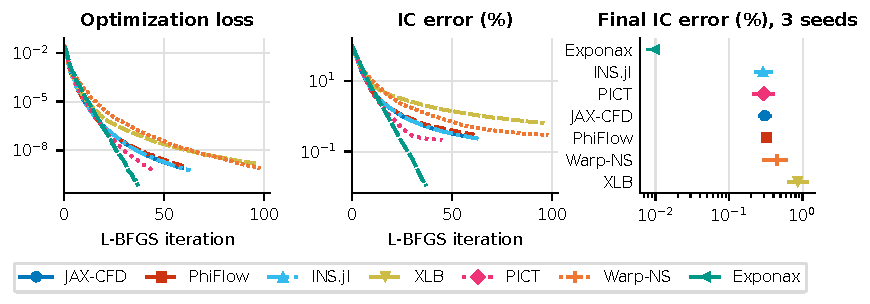
\includegraphics[width=\linewidth]{figures/recovery_main.pdf}
  \caption{F3 IC recovery with L-BFGS+proj. Left and middle: loss and IC error
    against iteration for the first target. Right: final IC error per solver,
    mean (dot) and range (bar) over three targets.}
  \label{fig:recovery_main}
\end{figure}

\begin{figure}
  \centering
  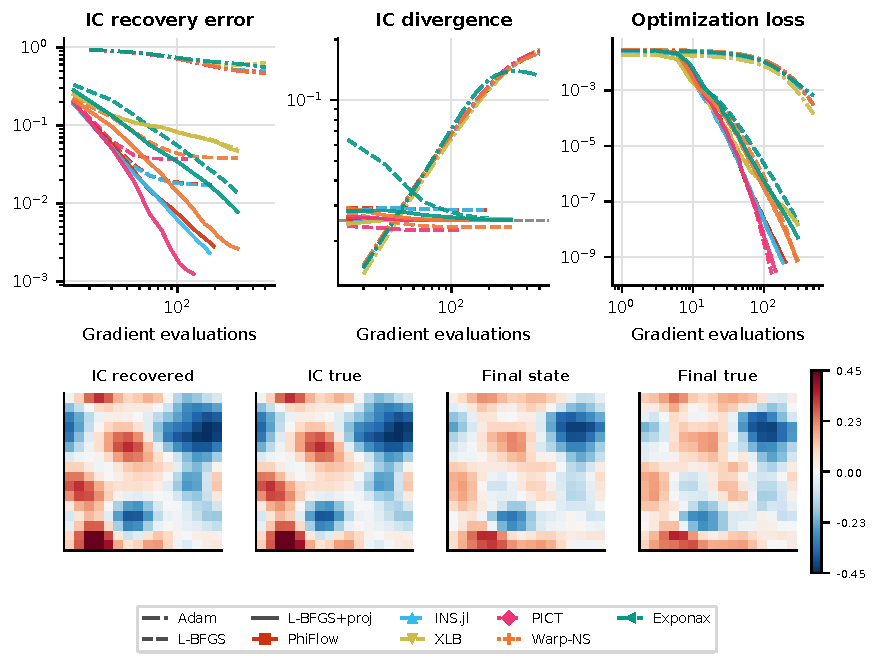
\includegraphics[width=\linewidth]{figures/recovery_overview.pdf}
  \caption{3D NS IC recovery overview for Adam, L-BFGS, and L-BFGS+proj (Adam+proj omitted; see \cref{fig:app:recovery:adamproj}).
    \emph{Top:} normalized IC error, IC divergence, and optimization loss vs.\ gradient evaluations across all solvers (color = solver, line style = optimizer).
    The dashed line marks the true IC divergence level.
    \emph{Bottom:} $u_x$ slice at convergence (L-BFGS+proj / PhiFlow): recovered IC, true IC, recovered final state, and true final state.}
  \label{fig:app:recovery}
\end{figure}

\begin{figure}
  \centering
  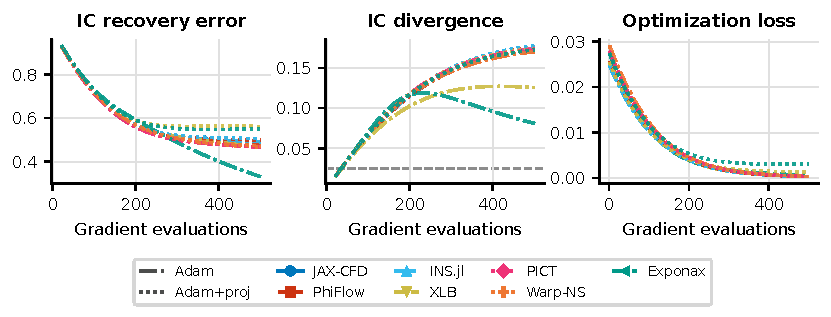
\includegraphics[width=\linewidth]{figures/recovery_adam_proj.pdf}
  \caption{Adam vs.\ Adam+proj on the 3D NS IC recovery task (linear scale).
    Adding a solenoidal projection step after each Adam update leaves IC error, IC divergence, and optimization loss essentially unchanged across all solvers, confirming that the projection benefit observed in \cref{fig:app:recovery} is specific to L-BFGS.}
  \label{fig:app:recovery:adamproj}
\end{figure}

\paragraph{Topology optimization}
\Cref{fig:app:topopt} summarizes the structural topology optimization task
($[0,2]\times[0,1]\times[0,1]$ cantilever beam, $16\times2\times8$ mesh, SIMP
with $p=3$). With Adam, the compliance of all five differentiable solvers
levels off after about 1\,460 of the 2\,500 iterations, and the final values
agree to seven significant digits ($1.003330\times10^{-3}$): for smooth,
well-conditioned physics, gradient quality does not limit solution quality.
The optimized density fields are visually identical across solvers, recovering
the classic cantilever-beam truss topology.

We also evaluated L-BFGS and MMA~\citep{svanberg1987mma} on this task.
After 100 quasi-Newton steps, L-BFGS final compliance ranged from $0.001$
(TopOpt.jl) to $0.008$ (JAX-FEM), well above the Adam solution. Two properties
of the problem plausibly explain this: the SIMP penalization ($p=3$) makes the
objective non-convex, so the curvature condition $y_k^\top s_k > 0$ required
for valid BFGS updates is often violated and updates are
skipped~\citep{fu2023quasinewton}; and the box constraints $\rho \in [0,1]$
cause rapid active-set changes that invalidate the limited curvature history.
MMA converged to a compliance of ${\approx}0.00099$ in about 40 iterations,
matching Adam's solution in under 2\% of its iteration budget, because it
builds a strictly convex separable approximation at each step and handles the
box constraints and the volume inequality natively. This agrees with standard
practice in topology optimization, where MMA is the usual choice.

\begin{figure}
  \centering
  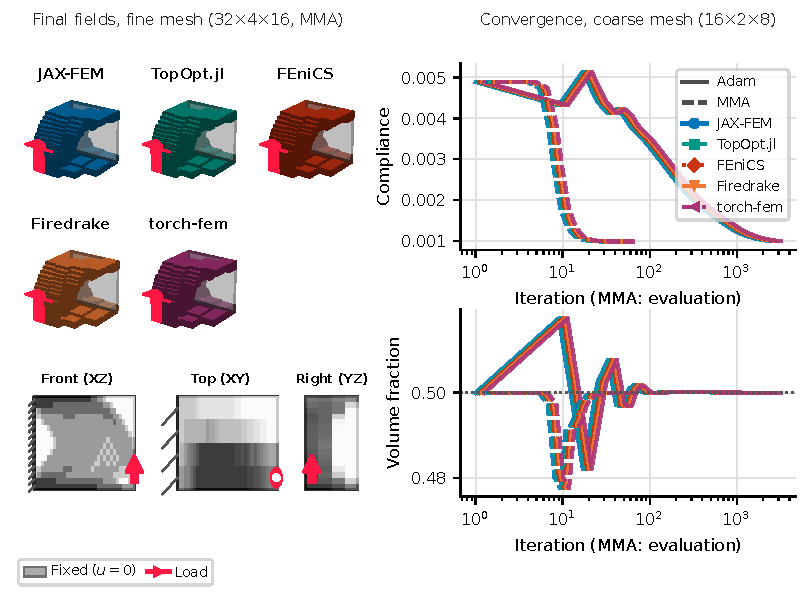
\includegraphics[width=\linewidth]{figures/topopt_overview.pdf}
  \caption{Structural topology optimization overview.
    \emph{Left:} final optimized density fields from a finer-mesh ($32{\times}4{\times}16$) MMA run, both as 3D voxel renderings (one per solver) and projected along each principal axis.
    \emph{Right:} compliance and volume-fraction vs.\ iteration for Adam and MMA (line style = optimizer, color = solver) on the coarser $16{\times}2{\times}8$ mesh used throughout the rest of the comparison; MMA converges in $\sim$40 iterations, Adam requires $\sim$2500.
    The two columns therefore use different mesh resolutions, as flagged in the panel headers: the finer run sharpens the recovered topology visually, while the coarser run keeps optimizer convergence directly comparable to the other tasks.}
  \label{fig:app:topopt}
\end{figure}

\paragraph{Conductivity recovery}
\Cref{fig:app:conductivity_recovery} shows the thermal conductivity inversion.
The ground-truth conductivity has two Gaussian peaks; each solver observes the
steady-state temperature under a known heat flux and recovers the conductivity
by minimizing the squared $\ell_2$ misfit between simulated and observed
temperatures. Starting from a uniform field, L-BFGS-B lowers the misfit of all
four solvers from $6.1\times10^{9}$ to 34--51 within 1\,000 iterations
(JAX-FEM 34, Firedrake 39, torch-fem 49, FEniCS 51), leveling off after
735--846 iterations. The recovered conductivity is 4.2--5.9\% from the truth in
relative $\ell_2$ norm, and the four recovered fields differ from each other by
1--3.5\% of the truth's norm. We attribute the spread to the poor conditioning
of the inversion: many conductivity fields fit the temperatures almost equally
well, and which one the optimizer reaches depends on its path. Consistent with
this, the same solver's final misfit differs by up to 21\% between the A100 run
and our T4 CI run.

\begin{figure}
  \centering
  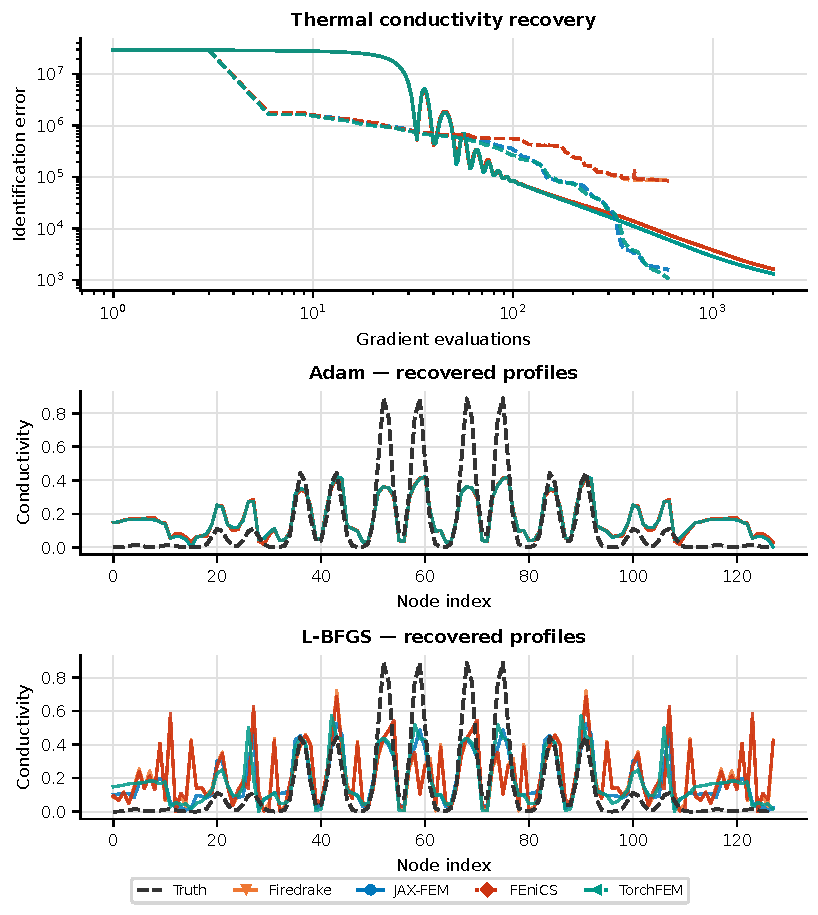
\includegraphics[width=\linewidth]{figures/conductivity_recovery_overview.pdf}
  \caption{Thermal conductivity recovery with L-BFGS-B. \emph{Top:} temperature misfit and relative error of the recovered conductivity against iteration, per solver. \emph{Bottom:} ground-truth and recovered conductivity fields.}
  \label{fig:app:conductivity_recovery}
\end{figure}

\subsection{Solver-in-the-loop study}
\label{app:sil}

\paragraph{Corrector}
A periodic CNN with three $5\times5$ convolutional layers and 8 hidden channels
reads the velocity and the phase of the forcing ($\sin\kappa y$,
$\cos\kappa y$), since the force breaks the translation symmetry in $y$. It
returns a stream function $\psi$, and the correction is its spectral curl, which
is exactly divergence-free with zero mean. The readout starts at zero, so an
untrained corrector leaves the solver unchanged. Input and output scales are
fixed by the forcing rather than by any solver's data, and every solver trains
the same architecture from the same initialization.

\paragraph{Training}
Each solver runs the coarse configuration of \cref{app:kolmogorov} ($64^2$,
$\Delta t = 0.01$) and is corrected every 0.1 time units. Its targets are its
own $256^2$ run from the ground truth's training states, restricted to $64^2$.
The three trained arms are \emph{supervised}, on fixed pairs (the solver's output
from reference frame $k$, and reference frame $k+1$) with no solver in the
training graph; \emph{stopped}, on a corrected 16-interval rollout with the
gradient stopped at every solver output; and \emph{SIL}, on the same rollout
differentiated through the solver. All arms see the same windows and use Adam
with learning rate $10^{-3}$ and global-norm clipping for 256 updates, for each
of three network seeds. The loss is the mean over the rollout of
$\|s - t\|^2 / \|t\|^2$, without per-solver normalization. Validation on a
separate state every 32 updates selects the checkpoint, with update 0, the
uncorrected solver, as a candidate. Every selected and final corrector is then
evaluated on the three test states for 40 intervals, and rolled out for 200
intervals to check stability.

\paragraph{Gates}
A solver is admitted if its $256^2$ reference differs from a $512^2$ run by at
most a quarter of the gap between its coarse run and the reference (observed
ratios 0.003 to 0.093), if chained calls reproduce one long call, and if the
gradient of the training loss through 16 intervals matches central finite
differences to within 5\% at a zero and at a random nonzero readout (observed
errors $1.2\times10^{-4}$ to $1.9\times10^{-3}$). All five solvers pass every
gate. Warp-NS and PhiFlow are not part of the study, for the reasons given in
\cref{app:kolmogorov}.

\paragraph{Native solver state}
For staggered and lattice solvers, a chain of calls that restarts from the
cell-centered velocity is a different map from one long call, because every
restart interpolates to the cell centers and back.
\Cref{tab:app:sil-closure} shows how far such chains drift. For the study,
JAX-CFD, INS.jl and XLB take and return their native state (face velocities or
lattice populations) as an optional input and output, which makes chains exact
up to round-off. PICT and Exponax are collocated and carry no history between
steps, so they restart exactly without it.

\begin{table}[h]
  \centering\small
  \caption{Closure of chained calls: median relative $\ell_2$ distance over the
    three test states between a chain of one-interval calls and one call over
    the same time.}
  \label{tab:app:sil-closure}
  \begin{tabular}{@{}lcccccc@{}}
    \toprule
    & \multicolumn{3}{c}{\textbf{Restart from velocity}} & \multicolumn{3}{c}{\textbf{Native state}} \\
    \cmidrule(lr){2-4}\cmidrule(l){5-7}
    \textbf{Solver} & 2 calls & 16 & 40 & 2 calls & 16 & 40 \\
    \midrule
    JAX-CFD & 1.0e-2 & 0.13 & 0.55 & 0 & 0 & 0 \\
    INS.jl & 1.0e-2 & 0.13 & 0.55 & 0 & 0 & 0 \\
    XLB & 5.3e-3 & 2.3e-2 & 9.7e-2 & 1e-6 & 1e-6 & 3e-6 \\
    PICT & 0 & 0 & 0 & $-$ & $-$ & $-$ \\
    Exponax & 1e-6 & 7e-6 & 5e-5 & $-$ & $-$ & $-$ \\
    \bottomrule
  \end{tabular}
\end{table}

\begin{table}[h]
  \centering\small
  \caption{Solver-in-the-loop results. Mean relative test error over 40
    intervals for each of the three network seeds, the uncorrected solver's
    error, and the wall time per training update at a 16-interval rollout. The
    runs partly shared the GPU with other jobs, so the times are rough.}
  \label{tab:app:sil}
  \setlength{\tabcolsep}{4pt}
  \begin{tabular}{@{}lccccc@{}}
    \toprule
    & \multicolumn{3}{c}{\textbf{Test error per seed}} & & \textbf{s / update} \\
    \cmidrule(lr){2-4}\cmidrule(l){6-6}
    \textbf{Solver} & Supervised & Stopped & SIL & Uncorrected & stopped / SIL \\
    \midrule
    JAX-CFD & 0.117 0.100 0.108 & 0.151 0.161 0.167 & 0.193 0.151 0.189 & 0.243 & 0.69 / 1.00 \\
    INS.jl & 0.117 0.100 0.108 & 0.151 0.161 0.167 & 0.193 0.151 0.189 & 0.243 & 0.87 / 2.35 \\
    Exponax & 0.068 0.075 0.067 & 0.063 0.061 0.065 & 0.076 0.068 0.063 & 0.091 & 0.75 / 1.02 \\
    XLB & 0.069 0.061 0.063 & 0.078 0.085 0.068 & 0.084 0.073 0.102 & 0.086 & 0.85 / 1.38 \\
    PICT & 0.145 0.143 0.147 & 0.186 0.169 0.150 & 0.228 0.161 0.192 & 0.277 & 4.73 / 26.8 \\
    \bottomrule
  \end{tabular}
\end{table}

\paragraph{Results}
All 45 trainings complete their 256 updates. The SIL arm's gradient norms are
10 to 20 times those of the stopped arm but stay bounded. None of the 270 long
rollouts turns non-finite, and no arm leaves a corrector less stable than the
uncorrected solver: the peak kinetic energy of a corrected rollout reaches 1.06
to 1.50 times the uncorrected mean, against 1.09 to 1.45 for the uncorrected
solver itself. Averaged over the seeds (\cref{tab:app:sil}), supervised training
gives the lowest error on every solver except Exponax, where the stopped arm is
lower, and SIL is never better than the stopped arm. On individual seeds it is.
Supervised updates take about 0.02\,s, since the solver's outputs for the pairs
are computed once in advance. JAX-CFD and INS.jl agree to every printed digit throughout, as
on the forward checks.

\paragraph{Reproduction}
The study is not part of the benchmark release. Its code, consisting of the
native solver state, the training experiment, a smaller version of it that
checks feasibility in minutes per solver, and the scripts that produce these
tables, is archived with the paper's reproduction materials.
% TODO: link the archived tag of pasteurlabs/mosaic#316 once it exists.


\section{Solver interventions}
\label{app:interventions}

Mosaic records every departure from a solver's default usage, so that a
reader can tell a solver used as documented from one whose wrapper works
around its limitations. This appendix describes the record format and the
rules around it, and reports an audit of all 19 solver wrappers in the
repository (commit \texttt{6517f75}, October 2026).

\subsection{Record format}

\begin{table}[h]
  \centering\small
  \caption{Intervention levels, assigned by mechanism. Examples are from the
    audit.}
  \label{tab:app:ladder}
  \begin{tabularx}{\linewidth}{@{}l l X@{}}
    \toprule
    \textbf{Level} & \textbf{Mechanism} & \textbf{Example} \\
    \midrule
    L0 & Documented options & MUMPS as FEniCS's forward linear solver \\
    L1 & Undocumented settings & An undocumented collision-operator switch threshold in XLB \\
    L2 & User code on public primitives & A custom pyadjoint block for a nodal misfit in FEniCS \\
    L3 & Changes to the solver & A monkeypatch of phiml's NumPy backend for 64-bit indices in PhiFlow \\
    L4 & Unreleased upstream fixes & Not accepted \\
    \bottomrule
  \end{tabularx}
\end{table}

\paragraph{Fields}
Each intervention records what was done, its level (\cref{tab:app:ladder}),
its necessity (required, a choice among library alternatives, or unknown),
whether its value was tuned by measurement, and, per setup, why it is
needed: the consequences of skipping it (the setup cannot be expressed, a
crash, non-finite output, an inaccurate forward solution, a missing or
incorrect gradient, an optimizer stall, excessive run time or memory, or
non-reproducible results), the symptom with a number where one exists, and
the evidence. Workarounds of upstream bugs link the upstream issue. Fixes to
Mosaic's own code, failure detection that changes no result, and build
infrastructure are not recorded. What counts as ordinary use depends on the
library's abstraction level: writing the assembly loop is ordinary use of
deal.II, and for a kernel toolkit such as NVIDIA Warp the hand-written solver
is the baseline, so only interventions made for the benchmark are recorded.

\paragraph{Policies}
(i) \emph{Choice of scheme.} A solver may run any scheme its library
offers. A non-default scheme is allowed when an experienced user of this
kind of simulator would pick it for the problem and a measurement shows its
gain; it is recorded as an intervention. Whichever scheme runs, its errors
are artifacts of the method and stay in the results.
(ii) \emph{Runtime adaptations.} Caches may hold state derived from inputs
that are not differentiable and from array shapes, never values derived from
differentiable inputs. One untimed warm-up call precedes the timed calls, and
its wall time is reported as the first-call cost. The same contract applies
to every solver.
(iii) \emph{Setup deviations.} A solver may substitute a documented
alternative for part of a setup it cannot express if it still passes the
setup's checks; the deviation is shown with its results.
(iv) \emph{Tuning.} Tuning is ordinary use and every solver receives it.
Tolerances are set to the loosest value at which every check of the setup is
unchanged, framework defaults are only disabled for reasons that reproduce on
the benchmark hardware, and cost is compared within a device class.

\paragraph{Rules}
Every solver runs on a released upstream version, or on a pinned commit where
the project has no releases. Upstream bugs are excluded by default; a
workaround links the upstream issue and is removed once a release fixes the
bug. A change to the discrete method itself, as opposed to how it is used,
creates a separate solver entry. An intervention shown to be unnecessary is
removed.

\subsection{Audit}

The audit used a first version of the format that recorded only the level.
\Cref{tab:app:audit} summarizes it.

\begin{table}[h]
  \centering\small
  \caption{Interventions found in all 19 solver wrappers, by level, by how
    well their reason is supported, and by the consequence of skipping
    them. \emph{Verified}: backed by a test, a measurement, or an upstream
    issue. \emph{Stated}: asserted in a code comment or pull request.
    \emph{Inferred}: no reason recorded.}
  \label{tab:app:audit}
  \begin{tabular}{@{}lr@{\qquad}lr@{\qquad}lr@{}}
    \toprule
    \multicolumn{2}{@{}l}{\textbf{Level}} & \multicolumn{2}{l}{\textbf{Reason}} & \multicolumn{2}{l@{}}{\textbf{Consequence}} \\
    \midrule
    L0 & 39 & Verified & 8 & Too slow & 27 \\
    L1 & 22 & Stated & 50 & Inaccurate forward & 17 \\
    L2 & 23 & Inferred & 34 & Crash & 14 \\
    L3 & 8 & & & Cannot express & 9 \\
       &   & & & Out of memory & 9 \\
       &   & & & Incorrect gradient & 8 \\
       &   & & & Other & 8 \\
    \bottomrule
  \end{tabular}
\end{table}

\paragraph{Findings}
The same need lands at very different levels across libraries. Running the
adjoint solve with MUMPS takes an L3 monkeypatch in FEniCS and nothing in
Firedrake; a nodal-sum misfit gradient takes a 78-line custom block in FEniCS
and 14 lines of documented API in Firedrake; the drag force is hand-written
(L2) in PICT and a documented function object in OpenFOAM. Asking for the
reason behind each intervention surfaced dead code, interventions that turned
out unnecessary, workarounds of upstream bugs that had never been reported,
comments whose stated reason did not hold, and departures from library
default schemes without a recorded measurement. It also showed that the
level alone is not enough: it conflates how something was done with whether
it was needed, it hides deviations from the prescribed setup, and what counts
as ordinary use depends on the library's abstraction level. Necessity, setup
deviations, and the abstraction-dependent baseline above were added in
response.

Resolving the findings changed several solvers after the pinned release, for
example running XLB with its default BGK collision operator, Exponax with its
default dealiasing, and PhiFlow with the schemes its documentation
recommends. These changes are published with the continuously updated
results; the tables in this paper reflect the pinned release.

\section{Solver documentation}
\label{app:solvers}

This appendix documents all solvers evaluated for inclusion in Mosaic,
covering implementation details, wrapping approach, and known limitations.
Solvers included in the benchmark appear in Table~\ref{tab:solvers}.
Excluded solvers and the reasons for their exclusion are listed in
\cref{app:excluded}.

\subsection{Included solvers}
\label{app:included}

\paragraph{JAX-CFD~\cite{kochkov2021machine}}
JAX-native incompressible flow solver on a staggered MAC grid with
finite-difference advection and spectral (FFT) pressure projection.
Gradients via JAX source-transformation AD.
The spectral pressure solve requires periodic BCs in all spatial directions,
so JAX-CFD is included in periodic benchmarks (TGV, multimode
agreement) but excluded from the cylinder-wake experiment.

\paragraph{PhiFlow~\cite{holl2024phiflow}}
Semi-Lagrangian advection with pressure projection.
Supports PyTorch, JAX, and TensorFlow backends, enabling gradient
computation through the same simulation code across AD frameworks.

\paragraph{INS.jl~\cite{agdestein2024ins}}
IncompressibleNavierStokes.jl: Julia finite-difference pressure-projection
solver. Differentiates through the time loop via Zygote.jl reverse-mode AD.
CPU only.

\paragraph{XLB~\cite{ataei2024xlb}}
JAX-native lattice Boltzmann solver supporting D2Q9 (2D) and D3Q27 (3D) stencils on
GPU. Gradients via source-transformation AD through the collision-streaming
loop.

\paragraph{PICT~\cite{franz2025pict}}
GPU-accelerated differentiable incompressible Navier--Stokes solver built on
PyTorch with custom CUDA kernels implementing the PISO algorithm. Supports
reverse-mode AD through the full time loop and handles multi-block
curvilinear grids. The Mosaic Tesseract exposes periodic, lid-driven cavity,
inflow/channel (with advective outflow), and cylinder-wake modes via an
8-block ring topology.

\paragraph{Warp-NS~\cite{macklin2024warp}}
Custom incompressible NS solver built with NVIDIA Warp CUDA kernels,
implementing the IPCS projection scheme with an FFT-based Poisson solve
(following a reference spectral example; a non-periodic solver was not
implemented). Gradients via the \texttt{wp.Tape} kernel-level VJP.
The Warp framework provides differentiable kernels but no ready-made
incompressible flow solver, so the FD stencils, pressure Poisson solve,
and time integration were implemented from scratch using Warp primitives.
Warp-NS represents a best-effort implementation by the Mosaic team and
illustrates the integration cost when a kernel toolkit provides no
built-in solver.

\paragraph{Exponax~\cite{koehler2024apebench}}
Spectral incompressible Navier--Stokes solver supporting both 2D
(streamfunction-vorticity) and 3D (Leray-projected velocity) formulations,
integrated with an exponential time-differencing Runge-Kutta (ETDRK) scheme.
Incompressibility is enforced to machine precision by construction.
Gradients via JAX source-transformation AD.
Used in Mosaic for the periodic setups of F2 and F3, and as the ground truth
of the Kolmogorov-flow checks (\cref{app:kolmogorov}).

\paragraph{FEniCS~\cite{farrell2013automated}}
Finite-element solver using P1 elements for thermal and structural problems.
dolfin-adjoint automates the discrete adjoint by replaying the forward tape.

\paragraph{Firedrake~\cite{rathgeber2016firedrake}}
Mirrors the FEniCS P1/CG1 formulation for structural and thermal problems.
Differentiates via firedrake-adjoint, providing an independent
tape-based adjoint implementation for cross-validation.

\paragraph{JAX-FEM~\cite{xue2023jaxfem}}
Solves heat conduction and linear elasticity with trilinear HEX8 finite
elements in JAX. Gradients via AD through the assembled system.

\paragraph{TopOpt.jl~\cite{huang2021topoptjl}}
SIMP topology optimization for linear elasticity with HEX8 elements in
Julia, using analytical adjoint sensitivities.

\paragraph{torch-fem~\cite{meyer2024torchfem}}
PyTorch finite-element solver for heat conduction with linear HEX8 elements.
Gradients via PyTorch autograd through the assembled system.
GPU-accelerated via PyTorch sparse operations.

\paragraph{OpenFOAM~\cite{weller1998tensorial} (reference)}
Runs the icoFoam incompressible PISO solver as a forward-only reference
baseline. No reverse-mode AD available.

\paragraph{deal.II~\cite{bangerth2007dealii,arndt2023dealii} (reference)}
Solves thermal and structural problems with Q1 elements using the
industry-grade C++ finite-element library.
No native reverse-mode AD is available; used as a forward-only reference
baseline for S and H, analogously to OpenFOAM for the fluid domains.

\subsection{Excluded solvers}
\label{app:excluded}

We document solvers that were evaluated for inclusion but ultimately
excluded, along with the specific reason in each case. Practitioners
looking for a particular solver can check whether it was considered and
why it was left out.

\paragraph{WaterLily.jl~\cite{waterlily2024}}
Forward-mode AD only, via \texttt{ForwardDiff.jl} dual numbers. No
Zygote reverse-mode support is documented. A VJP can be emulated by
contracting $N$ forward-mode JVPs, but the cost scales as
$O(N^d \cdot T_{\mathrm{fwd}})$, matching central finite differences.
Excluded from gradient benchmarks. Forward accuracy is reported where
applicable.

\paragraph{JAX-Fluids~\cite{jaxfluids2022}}
Targets compressible flow. Recovering the incompressible limit at low Mach
number ($\mathrm{Ma} \approx 0.01$) requires acoustic sub-stepping whose
iteration count depends on Ma, grid size, and time step simultaneously.
Because \texttt{jax.lax.scan} requires a statically known loop count, a
fully differentiable low-Mach wrapper cannot be built around the published
library without reimplementing its time integrator. Excluded from both
forward and gradient benchmarks.

\paragraph{Commercial solvers (ANSYS, COMSOL, Abaqus)}
Excluded for reproducibility: closed-source licenses prevent redistribution
of solver binaries or independent verification of gradient implementations.

\paragraph{FEniCS-NS~\cite{farrell2013automated}}
The FEniCS incompressible NS solver (CG1/CG1 elements, IPCS time-stepping)
was evaluated for fluid benchmarks but excluded for two independent reasons.
Without SUPG/GLS advection stabilization, stability requires
$\mathrm{Pe}_h = Uh/(2\nu) \lesssim 1$; at $\nu < 0.01$ on the $N=64$
benchmark grid, relative errors reach 31--212 while other solvers stay in
0.02--0.16.
Independently, wall-clock scaling is empirically $O(N^{2.45})$ in serial;
the VJP at $N=64$ takes 1248\,s, and the forward pass alone for the drag
optimization task ($N=32$, 400 steps) requires approximately 25{,}000\,s,
exceeding the 1200\,s HTTP watchdog by a factor of 40.
FEniCS remains included for structural and heat-transfer domains (H, S),
where neither constraint applies.

\subsection{Observed solver limitations}
\label{app:solver-issues}

The following limitations were identified during benchmarking and resulted
in task-specific exclusions. Solvers excluded globally are documented in
\cref{app:excluded}.

\paragraph{PICT: viscosity not differentiable in PISOtorch\_diff}
PISOtorch\_diff tracks autograd through velocity fields and boundary
conditions, but treats viscosity as a static scalar: passing a
\texttt{requires\_grad=True} tensor as the viscosity argument produces a
result with no \texttt{grad\_fn} (confirmed by direct inspection of the
autograd graph). Differentiation w.r.t.\ $\nu$ would require adding
viscosity as an explicit differentiable parameter inside the PISOtorch\_diff
C++/CUDA kernels; this is outside the scope of the Mosaic wrapper.

\paragraph{JAX-CFD: spectral pressure solve requires periodic boundary conditions}
JAX-CFD uses an FFT-based pressure Poisson solver that requires doubly-periodic
boundary conditions by construction. The 2D cylinder drag optimization
domain is a channel with inlet, outlet, and obstacle boundaries, none of
which are periodic. Volume penalization masks velocity inside the solid
region but does not remove the periodicity requirement from the pressure
solve. JAX-CFD is structurally excluded from the drag optimization task.

\paragraph{Warp-NS: no non-periodic pressure solver available within the time budget}
The Warp-NS implementation was built following a reference example that uses an
FFT-based spectral Poisson solver, which inherits the same doubly-periodic BC
requirement. Unlike JAX-CFD, this is not a structural limitation of the Warp
framework: a non-periodic iterative Poisson solver could in principle be
implemented using Warp primitives. However, no suitable example was available,
and implementing one from scratch was outside the time budget of this work;
the drag optimization was therefore not attempted.

\paragraph{INS.jl: viscosity gradient not available}
Zygote.jl cannot differentiate through the diffusion term in
IncompressibleNavierStokes.jl because its \texttt{ChainRulesCore} rule for
the diffusion operator returns \texttt{NoTangent()} for the viscosity
argument. Gradients w.r.t.\ $\nu$ are therefore not reported for INS.jl.
Fixing this requires either upstreaming a correct rrule into INS.jl or
implementing a custom adjoint that accounts for the diffusion term.

\paragraph{INS.jl: Brinkman penalization incompatible with spectral pressure solve}
INS.jl (IncompressibleNavierStokes.jl)~\cite{agdestein2024ins} supports periodic,
Dirichlet, symmetric, and advective outlet boundary conditions, but not
immersed boundary (IBM) or cut-cell methods. Applying Brinkman volume
penalization to represent the cylinder obstacle introduces a velocity
discontinuity at the solid boundary after each spectral LU pressure
projection step; the Poisson solve amplifies this discontinuity, and the
velocity field diverges to NaN at all tested resolutions ($N \geq 16$). A
correct approach requires incorporating the penalization term directly into
the pressure Poisson system~\cite{angot1999penalization}, which is outside
the scope of the current solver implementation. INS.jl is excluded from the
drag optimization task.

\paragraph{XLB: intrinsic $O(\mathrm{Ma}^2)$ compressibility error}
The D2Q9 BGK lattice Boltzmann method~\cite{qian1992lattice} recovers the
incompressible Navier--Stokes equations only to $O(\mathrm{Ma}^2)$ via
Chapman-Enskog expansion. At fixed $\Delta t$, the Mach number
$\mathrm{Ma} = u\,\Delta t / \Delta x$ grows with grid refinement, so the
compressibility error does not decrease with spatial resolution for
incompressible problems. At $N = 128$, $\Delta t = 0.01$,
$\mathrm{Ma} \approx 0.2$, giving an $O(0.04)$ error floor independent of
solver correctness~\cite{ataei2024xlb}. XLB forward accuracy results at
fine grids should be interpreted with this limit in mind.

\paragraph{XLB: BGK collision instability at low viscosity}
The BGK relaxation time $\tau = \nu/c_s^2\,\Delta t + 0.5$ approaches the
stability boundary $\tau \to 0.5$ as $\nu \to 0$~\cite{qian1992lattice}.
The XLB tesseract automatically selects the KBC (entropic) collision
operator~\cite{ataei2024xlb} when $\omega > 1.8$ ($\tau < 0.556$), which is
unconditionally entropy-stable.
Results at $\nu \in \{10^{-4},\, 5\times10^{-4}\}$ are pending re-validation
under the KBC operator and should be interpreted with caution.
